\documentclass{report}
\usepackage[T1]{fontenc} % Fontes T1
\usepackage[utf8]{inputenc} % Input UTF8
\usepackage[backend=biber, style=ieee]{biblatex} % para usar bibliografia
\usepackage{csquotes} % citações
\usepackage[portuguese]{babel} % Usar língua portuguesa
\usepackage{blindtext} % Gerar texto automaticamente
\usepackage[printonlyused]{acronym}
\usepackage{hyperref} % para autoref
\usepackage{url} % urlsites
\usepackage{graphicx} % introdução de imagens
\usepackage[table]{xcolor} % cor nas tabelas

%
\bibliography{bibliografia}
%
\begin{document}
%%
% Definições
%
\def\titulo{Spotify, cultura sonora 24/7}
\def\data{1º Semestre 2020}
\def\autores{Inês Santos, João Afonso Ferreira}
\def\autorescontactos{(103477) ines.santos20@ua.pt, (103037) ferreiraafonsojoao@ua.pt}
\def\versao{VERSAO}
\def\departamento{DETI}
\def\empresa{Universidade de Aveiro}
\def\logotipo{Imagens/ua.pdf}
%
%%%%%% CAPA %%%%%%
%
\renewcommand{\contentsname}{Índice}
\begin{titlepage}

\begin{center}
%
\vspace*{50mm}
%
{\Huge \titulo}\\ 
%
\vspace{10mm}
%
{\Large \empresa}\\
%
\vspace{10mm}
%
{\LARGE \autores}\\ 
%
\vspace{30mm}
%
\begin{figure}
\center
\includegraphics{\logotipo}
\end{figure}
%
\vspace{30mm}
\end{center}
%
\begin{flushright}
\versao 1
\end{flushright}
\end{titlepage}

%%  Página de Título %%
\title{%
{\Huge\textbf{\titulo}}\\
{\Large \departamento\\ \empresa}
}
%
\author{%
    \autores \\
    \autorescontactos
}
%
\date{\data}
%
\maketitle
%
\pagenumbering{roman}
%
\tableofcontents % índice
\listoffigures % lista de figuras
\listoftables % lista de tabelas

%%%%%% RESUMO %%%%%%
\begin{abstract}

No âmbito da Unidade Curricular anual de Laboratórios de Informática do $1^{o}$ ano do curso de~\ac{miect}, decidimos abordar uma temática sempre presente na vida de qualquer um de nós que é a ``música''. Mais concretamente, a forma como hoje em dia a ouvimos de forma rápida, em qualquer lugar e em qualquer instante através dos nossos dispositivos móveis e ultra-móveis, como é o caso dos nossos \emph{smartphones}. Este actual ``milagre'' tecnológico é hoje conseguido através dos actuais serviços de \emph{audio-streaming} onde o \emph{Spotify} é aquele que nos parece ser o mais usado pelas massas ao permitir usufruir de conteúdo sonoro de forma extremamente intuitiva e a um custo bastante apelativo.

Numa primeira abordagem, decidiu-se começar por introduzir o impacto que estas plataformas têm ao moldar a cultura de cada pessoa, contextualizando um pouco da história desta empresa sueca, o seu surgimento e objetivos a que se propôs desde início. De seguida, enumera-se e descreve-se algumas das funcionalidades que tornam esta aplicação única e líder no mercado. %Ao longo deste estudo iremos também fornecer informação sobre outras empresas, tanto concorrentes como parceiras, que enaltecem ainda mais a abundância de conteúdo musical existente em todo o mundo, sob a forma de plataformas digitais de \textit{streaming} acessíveis a qualquer um que queira tirar partido das mesmas.

Em suma, pretende-se fazer uma análise das principais funcionalidades do \textit{Spotify}, assim como de algumas técnicas de marketing usadas para continuar a obter uma crescente aderência por parte da população mundial. Além disso apresentamos alguns dados estatísticos e fortes indícios, obtidos pela revisão bibliográfica,  que de facto esta plataforma ainda se encontra  em crescimento.

Por fim, fazer-se-á uma reflexão sobre os aspetos abordados ao longo deste trabalho, incluindo considerações acerca do futuro (próximo) desta revolucionária empresa de conteúdo digital.

\end{abstract}



%%%%%% Agradecimentos %%%%%%
\renewcommand{\abstractname}{Agradecimentos}
\begin{abstract}

Queremos, desde já, agradecer ao docente António Manuel Adrego da Rocha da \ac{ua}, por ter sido prestável ao nível do esclarecimento de qualquer dúvida em eventuais aspetos técnicos deste trabalho.

\end{abstract}
%
\clearpage

\pagenumbering{arabic}

%%%%%%%%%%%%%%%%%%%%%%%%%%%%%%%%
\chapter{Introdução}
\label{chap.introducao}

\begin{quote}
``\emph{A arte existe para que a realidade não nos destrua.}''
\end{quote}
\begin{flushright}
Friedrich Nietzsche
\end{flushright}

% Pergunta de partida - qual a pergunta de investigação: Será que o Spotify é a plataforma digital de áudio de alta qualidade mais usada? E porquê?

Desde sempre que a Música faz parte da nossa forma de viver, de estar, de nos transcendermos, como seres inteligentes e, desta forma, de nos abstrairmos da real dureza que é a Realidade. Por outro lado, a Música, considerada a rainha de todas as formas de Arte, também é capaz de juntar multidões, interligar vidas e criar revoluções sociais. Sem dúvida que a Arte, e em especial a Música, é uma das formas inequívocas que nos distingue dos outros seres vivos e sinónimo de Inteligência \ldots

Mas ouvir música nem sempre esteve à distância de um clique, visto que num passado não muito longíquo (estaremos a falar de cerca de duas décadas) as pessoas tinham de recorrer a leitores de cassetes, um disco de vinil num gira-discos ou, ainda mais atrás no tempo, a um cartucho (uma espécie de cassete, porém com um tamanho superior - esta é a frase mais usada pela publicidade do Stoptify!) para conseguir ouvir música. Estas maneiras clássicas, hoje em dia consideradas já \textit{vintage}, usadas para se ouvir música, embora revolucionárias na altura, traziam certas desvantagens como o tempo despendido ao acesso não imediato dos conteúdos musicais que se procurava desfrutar.

Ouvir música e o tipo de música que se ouve diz bastante da personalidade e história de cada pessoa, uma vez que esta tem o poder de despertar emoções e ter um efeito bastante poderoso tanto a nível físico como a nível psicológico, estando isto comprovado cientificamente~\cite{donaldahodges2000}.

%\begin{quote}
%``\emph{Music is an agreeable harmony for the honor of God and the permissible delights of the soul.}'' - Johann Sebastian Bach
%\end{quote}

Nos dias de hoje, existem plataformas inovadoras que foram criadas efetivamente para resolver estes constrangimentos. Ouvir música, rádio, podcasts, ou vídeo-podcasts nunca foi tão imediato, e é graças à existência destas novas plataformas digitais de streaming, que apenas requerem uma ligação à Internet, que as pessoas de todo o mundo têm a possibilidade de encontrar interesses em comum e usufruir do conteúdo que querem, quando assim o desejarem. 

O \textbf{Spotify} é uma dessas plataformas, criada em 2006 por \textit{Daniel Ek} e por \textit{Martin Lorentzon} capaz de trazer às massas uma ampla base de dados de música de todos os géneros cuja qualidade de serviço tem vindo a crescer ao longo dos anos e espelhada na forma como também tem vindo a ter cada vez mais utilizadores. Como é possível observar na Fig.~\ref{Fig:DesktopSpotify}, a atual versão da aplicação para desktop apresenta um tipo de aparência cuidada e bastante apelativa.

\begin{figure}
    \centering
    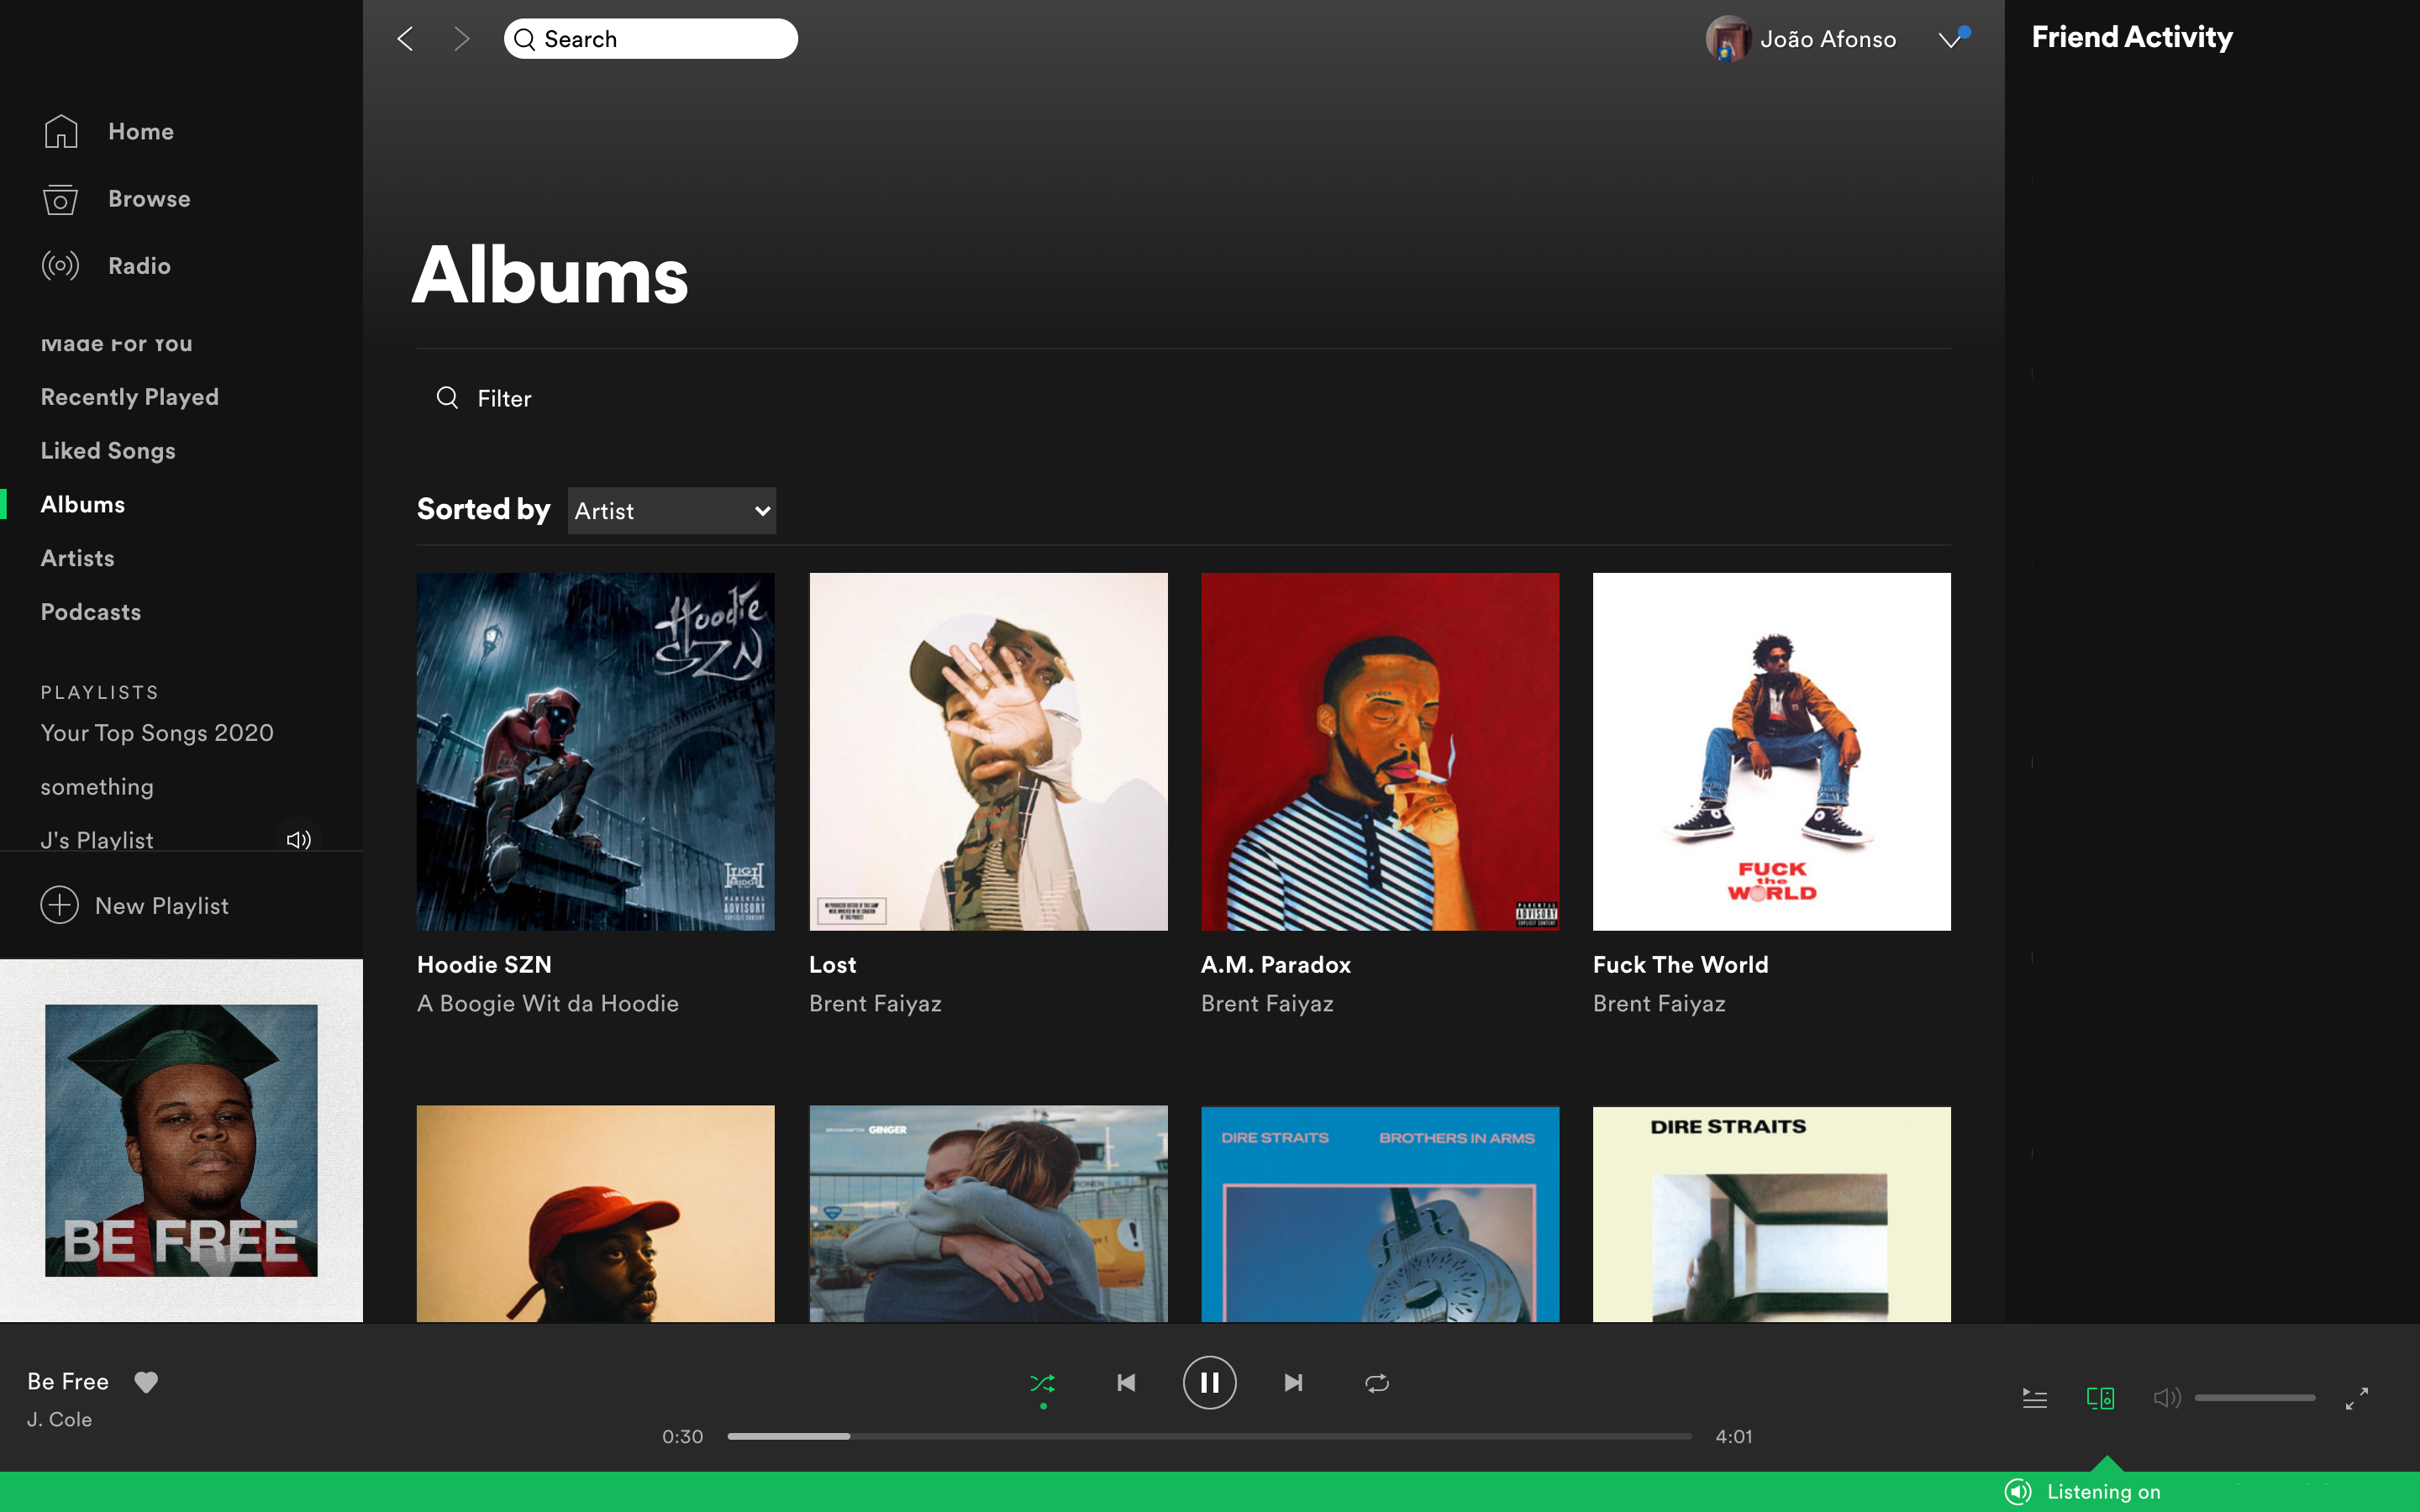
\includegraphics[width=\textwidth]{Imagens/DesktopSpotify}
    \caption{Versão desktop da aplicação Spotify.}
    \label{Fig:DesktopSpotify}
\end{figure}

Apesar do \textbf{Spotify} ser mais usada na sua versão ``\textit{freemium}'', em que o modelo de negócio acenta na publicidade constantemente apresentada de forma aleatória e sem qualquer controlo do utilizador final, como em muitas outras aplicações de \textit{streaming}, também apresenta  uma versão \textit{Premium} (versão paga) onde a publicidade é retirada e omitida.

Aparentemente esta \textit{app} parece dominar o mercado da indústria musical online onde, globalmente, tem mais de cerca de 100 milhões de utilizadores com a versão \textit{premium}, e diferenciando-se da concorrente mais próxima - \textit{Apple Music} com mais 50 milhões de subscritores~\cite{NuscaEtAll:2019}. Mas será ainda de facto?

\section{Objetivos}
Com este trabalho pretende-se obter respostas às seguintes perguntas de investigação: ``Será que o Spotify é a plataforma digital de áudio de alta qualidade mais usada e a mais usada pelo público em geral? E porquê?''

Com base nestas duas perguntas pretende-se assim estudar e caracterizar uma das aplicações de áudio-streaming mais conhecida - o Spotify.


\section{Organização do relatório}
Assim sendo, este documento está dividido em cinco capítulos. 
Neste primeiro, é feito uma contextualização sobre a forma como ouvimos música hoje em dia, seguida de uma pequena apresentação de uma das possíveis soluções de audio-streaming mais usada - o ``Spotify''. No \autoref{chap.funcionalidades} serão apresentadas algumas funcionalidades/características da aplicação, bem como a comparação com outras plataformas de ``audio-streaming''. O \autoref{chap. Críticas e aspetos polémicos} apresenta algumas críticas em termos dos aspetos menos ``positivos'' do Spotify reconhecidos pelos utilizadores como pelos criadores de conteúdo. No \autoref{chap.Técnicas de Marketing e publicidade da empresa} serão apresentadas algumas técnicas de Marketing e Publicidade da empresa, bem como parcerias com outras empresas e algumas curiosidades interessantes.
Por fim, no \autoref{chap.conclusao}, apresentam-se as principais conclusões deste trabalho, contrapondo os objectivos inicialmente apresentados, e abordar-se-á de forma geral as potencialidades desta aplicação (Spotify), dando ênfase ao modo como prevemos que irá crescer num futuro não muito longínquo.

%\begin{quote}
%``\emph{We see the future not as something out of our control, but as something we can shape for the better through concerted and collective effort.}'' - Barack Obama
%\end{quote}


\chapter{Funcionalidades do Spotify}
\label{chap.funcionalidades}
\begin{quote}
``\emph{With Spotify, it’s easy to find the right music or podcast for every moment – on your phone, your computer, your tablet and more.}''
\end{quote}
\begin{flushright}
\emph{in} \url{https://www.spotify.com/pt/about-us/contact/}
\end{flushright}

Neste capítulo apresenta-se algumas funcionalidades/características da aplicação.

\section{O Spotify}
O Spotify é caraterizado pela sua interface gráfica intuitiva que permite a qualquer pessoa um fácil e rápido entendimento de como tirar partido da aplicação. Disponível para desktop, para vários sistemas operativos - MS-Windows, GNU/Linux ou macOS, também está disponível para tablets/iPads, televisões e smartphones (Android e iOS). Até nas consolas de jogos podemos encontrar esta aplicação que possui inúmeras funcionalidades extremamente úteis e que permitem aos utilizadores explorar a fundo e, muitas vezes, descobrir artistas ou géneros musicais (entre outros conteúdos) que de outra forma não chegariam até eles.

Tirando partido da versão Premium (a qual será, por defeito, a versão mais referida neste relatório), ao fazer login, os utilizadores deparam-se com um menu que coloca ao seu dispor, e de forma bem organizada, os conteúdos sonoros que recentemente se encontravam a ouvir, e que por alguma razão interromperam. A qualquer momento, podem retomar a música ou o podcast exatamente onde pararam de ouvir, inclusivamente se quiserem ouvir num outro dispositivo; por exemplo, se se encontravam a ouvir no computador e acharem em algum momento que preferiam estar a ouvir no telemóvel, é possível fazê-lo, e para tal, basta fazer o login pessoal nesse dispositivo, e selecionar a opção de conectar ao dispositivo que se pretender e estiver disponível. Desse modo, poderá ouvir o que estava a ouvir, no exato segundo onde parou, no aparelho que entender, e sem problemas de continuidade.

\section{A interface de utilizador}
A aplicação encontra-se dividida em 3 áreas principais: 
\begin{enumerate}
    \item A área de pesquisa
    \item A ``\textit{library}''/biblioteca pessoal
    \item A ``\textit{home}'' ou área inicial.%para ser possível mudar de página
\end{enumerate}

Na área de pesquisa, existe uma barra de pesquisa onde cada um pode inserir o nome de uma música que queira, de um \textit{podcast}, de um artista, ou de uma \textit{playlist} em específico. No entanto, também pode optar por selecionar uma das opções pré-estabelecidas pelo algoritmo desta área, que se encontra dividida pelos principais géneros musicais que ouve, ou por múltiplas outras alternativas de escolha que de certeza serão do agrado de alguém que não tenha uma ideia específica do que deseja ouvir num determinado momento. Existe também uma parceria muito interessante com a aplicação \textit{Shazam}, sendo que esta útlima é uma aplicação muito popular e que auxilia na descoberta de canções. Basta fornecer acesso ao microfone do telemóvel que, deste modo, ``ouve'' a música que se pretende decifrar e descobrir, e segundos depois (se disponível), é dada a essa pessoa a informação sobre essa música em específico. A parte interessante disto é que, se for feita a associação desta aplicação com a conta do \textit{Spotify} desse utilizador, será possível fazer a recolha das músicas descobertas e reencaminhá-las a todas diretamente para uma \textit{playlist} apenas com essas mesmas músicas.

\paragraph{} 

De certa forma, a biblioteca pessoal é um inventário pessoal de tudo o que um utilizador pretende guardar para futura audição e está também dividida nos espaços para Música e \textit{Podcasts}.
\begin{itemize}
    \item No espaço musical, tem-se: a lista de \textit{playlists} guardadas ou formadas pelo cliente; a lista dos artistas que o utilizador optou por seguir; e os álbuns guardados, dos artistas que se pretender.
    \item Já no espaço dos \textit{podcasts}, existe: a divisória onde é possível ver que episódios de um determinado \textit{podcast} se está presentemente a ouvir, e por baixo, os episódios dispostos por ordem cronológica (o mais recente na parte superior) de lançamento; a divisória dos downloads, onde se encontram os episódios de certos \textit{podcasts} que foram descarregados para, eventualmente, serem ouvidos sem recorrer à \textit{internet}; e a terceira divisória, onde se encontram os programas/\textit{podcasts} guardados, das pessoas que se escolheu seguir.
\end{itemize}

Voltando à ``\textit{home}'', na página inicial encontram-se dispostos vários conteúdos que, se prestarmos bem atenção, são-nos bastante úteis e que, com as técnicas algorítmicas desenvolvidas pelos engenheiros de software da empresa, chegam até nós de forma inesperada, mas certeira. 

À medida que uma pessoa vai ouvindo mais e mais, vai estabelecendo um certo perfil específico de géneros musicais que prefere ouvir, que estilo de artistas ouve, que \textit{playlists} mais a caracteriza, ou que estilos de \textit{podcasts} a definem como ouvinte. Digamos que estes pormenores são captados e são formadas secções nesta área inicial que acumulam pormenorizadas sugestões.

Estas secções contêm, por exemplo, \textit{playlists} feitas especificamente para o utilizador em questão, sendo as mais conhecidas as chamadas \textit{\textbf{“Daily Mixes”}}, com músicas selecionadas por géneros e artistas semelhantes, que são apresentadas de forma a aumentar o reportório de conhecimento musical dessa pessoa. Estas recomendações são feitas utilizando sistemas de inteligência artificial para filtrar os gostos dos usuários e criar recomendações personalizadas.

\paragraph{} 

Além destas \textit{playlists} personalizadas, existem muitas outras, das quais se destacam aqui, por exemplo, a \textit{\textbf{“Discover Weekly”}} (onde se captam novas músicas que surgem semanalmente), a \textit{\textbf{“Release Radar”}} (onde se faz um apanhado dos lançamentos dos artistas que o utilizador segue, com singles escolhidos de forma exclusiva),a \textit{\textbf{“On Repeat”}} (onde se agregam as músicas que se está predominantemente a ouvir numa determinada altura), a  \textit{\textbf{"Summer Rewind"}}, que retoma as músicas mais ouvidas num verão e muitas mais deste género.

 De forma similar, são também recomendadas \textit{playlists} já existentes baseadas no que se ouve recentemente e, no final de cada ano, é feito um apanhado das estatísticas pessoais de cada um, como que um histórico de memórias desse ano de utilização da aplicação, e com isso vem sempre uma \textit{playlist} com as 100 músicas mais ouvidas desse ano, a qual poderá ser guardada na biblioteca pessoal.
 
 Neste particular tema, é relevante constatar a parceria da \textit{Spotify} com uma plataforma de dados e inteligência musical chamada \textit{Echo Nest}. Comprada pela \textit{Spotify} em 2014, o seu campo de ação centra-se no facto de ajudar a \textit{Spotify} a curar \textit{playlists} de recomendação personalizadas com algoritmos que prevêm os estilos que os subscritores irão mais apreciar, desenhando o chamado \textit{Taste Profile}, baseando-se nos padrões de utilização de cada usuário. Inicialmente, a companhia \textit{Echo Nest} tinha por objetivo perceber o conteúdo áudio e textual da música, desenvolvendo técnicas de identificação musical, “audio \textit{fingerprinting}” e sugestão musical que foram posteriormente postas em prática aquando da parceria com a \textit{Spotify} a partir de 6 de março de 2014.

Abandonando o tópico popular das\textit{playlists}, é comum também nesta plataforma que se conecte a conta do \textit{Spotify} com uma rede social como o \textit{Facebook} e ouvir músicas não em privado, mas com amigos, podendo assim haver uma partilha imediata dos favoritos de cada um e uma troca cultural muito mais rica e em comunidade.

Estas são algumas das funcionalidades predominantes e mais conhecidas desta aplicação, das quais milhões de pessoas ao redor do mundo tiram partido e usufruem, criando-se uma rede de conectividade constantemente crescente.


\chapter{Críticas e aspetos polémicos}
\label{chap. Críticas e aspetos polémicos}


Neste capítulo apresenta-se algumas críticas em termos dos aspetos menos ``positivos'' do Spotify reconhecidos pelos utilizadores como pelos criadores de conteúdo.

\section{Críticas}
Embora esta plataforma seja indubitavelmente a dominante no mercado de consumo de cultura musical, não é tudo um mar de rosas... Esta empresa é pontualmente alvo de críticas significativas, nomeadamente no modo como trata os artistas. É polémico o facto de o \textit{Spotify} não pagar diretamente aos artistas por reprodução – devido à metodologia específica de pagamento por subscrição dos clientes, das \textit{Royalties} (pagamentos que são feitos aos artistas detentores dos conteúdos que lhes dá o direito de fazer \textit{stream} de músicas que pertencem a outrem) – até porque, por vezes, estes ainda têm que suportar comissões de 30\% sobre os seus contratos com editoras e \textit{labels}. De acordo com uma fórmula especifíca(~\ref{fig3:Royalties}), calcula-se que estes obtenham efetivamente apenas uma percentagem de cerca de 25\%.

Deste modo, as receitas que chegam aos artistas e produtores não são suficientemente elevadas, embora os \textit{Premium users} (utilizadores com a versão paga da aplicação) existam em grande número. Os que não usufruem deste serviço e ouvem os conteúdos a seu gosto de forma gratuita, não contribuem significativamente para a receita dos artistas. O \textit{Spotify} paga cerca de 52\% do lucro às editoras, que irão pagar aos artistas uma percentagem desde 15\% a 50\% desses 52\% das receitas, dependendo da dimensão do artista. E esta fórmula não chega a aplicar-se aos\textit{podcasts}, cujo lucro será ainda menor. Personalidades como a \emph{Taylor Swift} já demonstraram o seu descontentamento com a empresa, argumentando precisamente com o facto de esta não valorizar ou respeitar o trabalho dos artistas que possuem conteúdo na sua plataforma. 
Houve inclusive uma petição em março de 2020 para aumentar o preço das \textit{Royalties} aos artistas, devido à impossibilidade de realizar espetáculos em tempos de pandemia. 

Uma recente proposta polémica do \textit{Spotify} sobre este tema consistiu em uma oferta de propaganda adicional ao trabalho dos artistas (gerida por técnicas algorítmicas), em troca de cortes nas suas \textit{Royalties}. Esta proposta não foi recebida de forma amigável por parte da comunidade artística, sendo evidente que este é ainda um obstáculo a enfrentar pela empresa.

Obviamente, como qualquer outra empresa, \textit{Spotify} não foge à regra na competição para melhor plataforma de \textit{streaming} musical. Como tal, a concorrência consiste nas seguintes plataformas: \textit{SoundCloud}, \textit{iTunes/ Apple Music}(com uma base de clientes fiel, sendo a mais forte competição), \textit{Tidal} (possui influentes acionistas, como a \emph{Beyoncé}, o \emph{Jaz-Z} e a \emph{Madonna}…), \textit{Deezer}, \textit{Youtube Music} ~\cite{manuelpestanamachado2018}, entre outras . . . No entanto, a plataforma com maior êxito é, efetivamente, o \textit{Spotify}, por se destacar na diversidade de conteúdo disponibilizado aos seus \textit{users}.

%
\begin{figure}
    \centering
    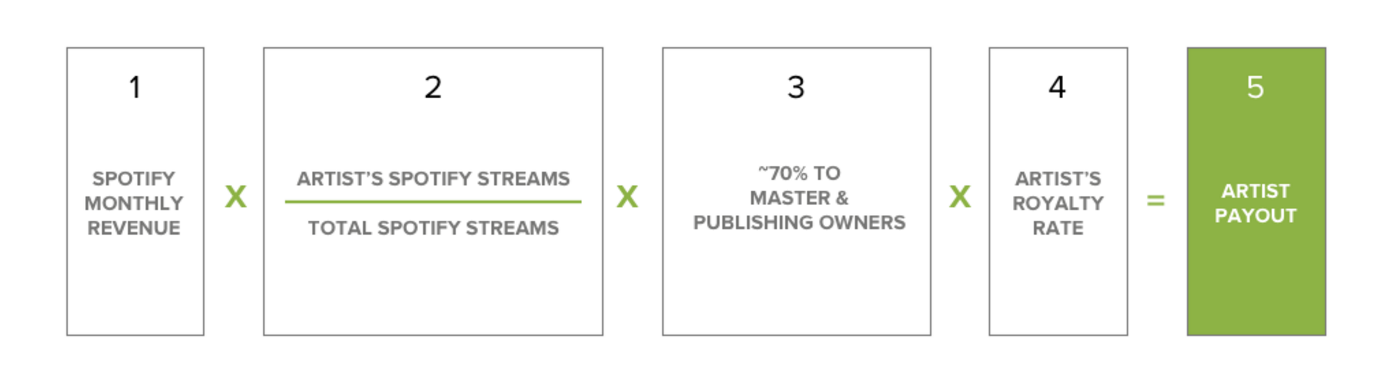
\includegraphics[width = \textwidth]{Imagens/royalties.png}
    \caption{Royalties} \label{fig3:Royalties}
\end{figure}
%

\section{Relação com a Pirataria}

Há contudo um aspeto importante a ter em consideração, que é o aspeto controverso da existência de pirataria. Ora, a própria criação da empresa teve como pilar o combate a esta prática recorrente nos anos 2000, e desde o seu lançamento em 2006 e a criação da aplicação em 2008, que os números de pirataria têm verdadeiramente vindo a diminuir, havendo um decréscimo notório de 55\% na pirataria por parte da faixa etária dos 18 aos 29 anos. Isto deve-se ao facto de o \textit{Spotify} ser acessível a todos e gratuito inicialmente, sendo que muitas vezes acontece uma gradual transição do estado gratuito para a subscrição \textit{Premium}, que acarreta substanciais vantagens tanto para os utilizadores como para os trabalhadores/administradores da empresa. 

Em suma, apesar das críticas e de toda a constante/crescente competição com plataformas como a \textit{Apple Music}, o \textit{Spotify} permanece no topo das plataformas de conteúdo sonoro digital, embora ainda não tenham sido maioritariamente enfrentadas as dificuldades de pagamento injusto aos artistas (causadas pela falta de transparência nessa relação burocrática e outros aspetos) e não se tenha em elevada consideração o facto de ser uma das empresas que contribuiu para o decréscimo da pirataria \textit{online} de músicas~\cite{tiagomonteiro&miguelmonteiro&joãofranco2019}.



\chapter{Técnicas de Marketing e publicidade da empresa}
\label{chap.Técnicas de Marketing e publicidade da empresa}
Neste capítulo apresenta-se algumas técnicas de Marketing e Publicidade da empresa, bem como parcerias com outras empresas e algumas curiosidades interessantes.

\section{Comparações com outras plataformas}
O \textbf{Spotify} é, sem dúvida, a melhor plataforma de \textit{streaming} em termos de números, segundo~\cite{mansooriqbal2000} e a fig.~\ref{fig6:mercado}. Já em 2008, quando foi lançada a aplicação, esta disparou exponencialmente graças à parceria que mantinha com o \textit{Facebook}, a maior companhia de redes sociais do mundo, e foi um enorme sucesso. Esta \textit{app} estreou-se publicamente em abril desse mesmo ano e no dia de estreia arrecadou um total de 26.5 mil milhões de dólares, um número excepcional. De momento é possível comprovar esta fama com os seguintes dados:

\begin{itemize}
  \item Spotify chega a um total de 320 milhões de utilizadores~\cite{visão2020}.
  \item 286 milhões de utilizadores ativos mensalmente.
  \item 130 milhões destes utilizadores mensais são subscritores Premium~\ref{fig5:stats}.
  \item Existem por volta de 50 milhões de músicas na plataforma
  \item A receita anual em 2019 foi de 6,7\$ biliões, com lucro bruto de 1,7\$ biliões
  \item o preço de mercado do \textit{Spotify} no início de maio de 2020 era de 26,9\$ biliões~\cite{mansooriqbal2000}. 
\end{itemize}

É de notar que na América, mais concretamente nos Estados Unidos, a popularidade da plataforma é efetivamente maior que a da a \textit{Apple Music} como comprova a Fig.~\ref{fig4:popularidade}. Muitas vezes, esta popularidade é não é transparecida através dos artistas, devido ao facto do valor por eles recebido no \textit{Spotify} ser menor ao valor recebido por eles através da \textit{Apple Music} (0,00348\$ < 0,00675\$ por cada reprodução).\\

\definecolor{caribbeangreen}{rgb}{0.0, 0.8, 0.6}

\begin{table} [h]
    \centering
    \begin{tabular}{|c|>{\columncolor{caribbeangreen}}c|c|c|}
        \hline
        \textbf{Apple Music} & \textbf{Spotify} & \textbf{Tidal} & \textbf{Youtube Music} \\ \hline
        256kbps     & 320kbps & 1411kbps & 128kbs \\
        \hline
    \end{tabular} \label{audio}
    \caption{Comparação de qualidade sonora}
\end{table}


Fazendo uma \textbf{comparação} direta entre o \textit{Apple Music} e \textit{Spotify} (fig.~\ref{fig:comparação}), é de notar as semelhanças e diferenças entre estas \textit{apps}. Começando pelo preço mensal por indivíduo, as duas rondam os 10 dólares americanos por mês, já no plano familiar há uma diferença (neste plano a \textit{Apple Music} favorece mais), uma vez que o preço para 6 pessoas é de 15 dólares americanos. Já no Spotify, são 5\$ por pessoa o que pode chegar aos 30\$ caso sejam 6 pessoas, ou seja o dobro comparativamente com o Apple Music. 
A \textit{Apple Music} distingue-se na qualidade de som no formato \textbf{grátis}(seção~\ref{audio}). Já na qualidade do formato premium é dificil de avaliar qual o melhor, uma vez que depende dos hábitos do ouvinte~\cite{davehenry2020}. 
No período experimental de subscrição é igual dos dois lados: 3 meses sem custos. Porém, no caso da Apple é necessário introduzir os dados de cartão multibanco antes de aderir a este período a que se tem direito, ao contrário do Spotify, em que basta registar uma nova conta. Outro aspeto importante é o desconto de estudante que apenas o Spotify possui, rondando os 5\$ americanos de desconto. Na aplicação do Spotify é possível fazer \textit{playlists colaborativas}, isto é, mais do que uma pessoa pode adicionar músicas a uma única playlist e ainda é possível ver o que os amigos estão a escutar num determinado momento, tudo isto ao contraponto com a \textit{Apple Music}, que não possui nenhuma destas duas funcionalidades. E ainda, é possível realçar o Spotify pela positiva apresentando o conceito de \textit{podcast}, isto é, um programa na forma de áudio ou vídeo, que ao contrário da rádio (por esta ser ao vivo), fica disponível na plataforma, sendo possível ouvir quando for conveniente para cada pessoa, sendo que a \textit{Apple Music} fica mais uma vez atrás do \textit{Spotify}.

% 
\begin{figure}
    \centering     
    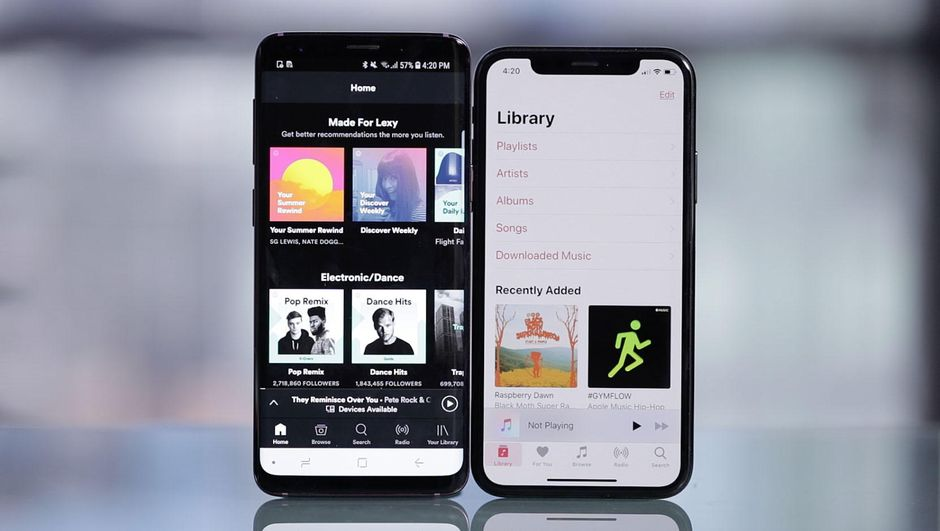
\includegraphics[width=\textwidth,height=60mm]{Imagens/applemusic-spotify.jpg}     
    \caption{Spotify versus Apple Music} 
    \label{fig:comparação} 
\end{figure}
%

\begin{figure}
    \centering
    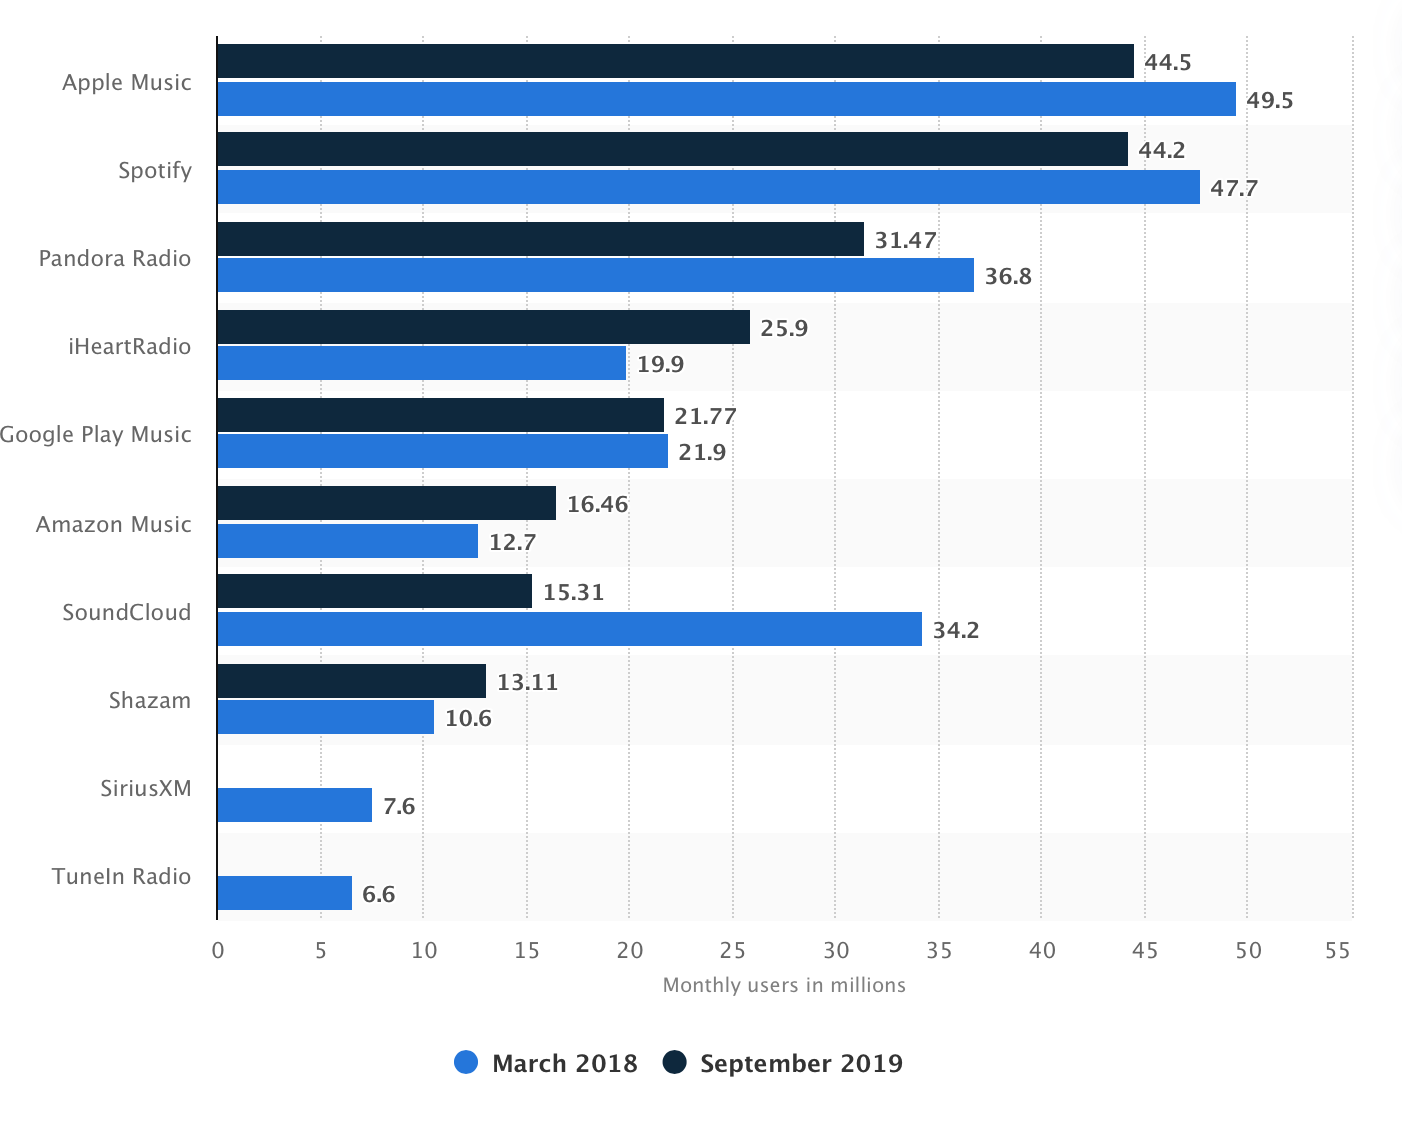
\includegraphics[scale = 0.4]{Imagens/Most popular music streaming services in the United States in March 2018 and September 2019, by monthly users.png}
    \caption{As plataformas mais populares nos USA} \label{fig4:popularidade}
\end{figure}
%
\begin{figure} 
    \centering
    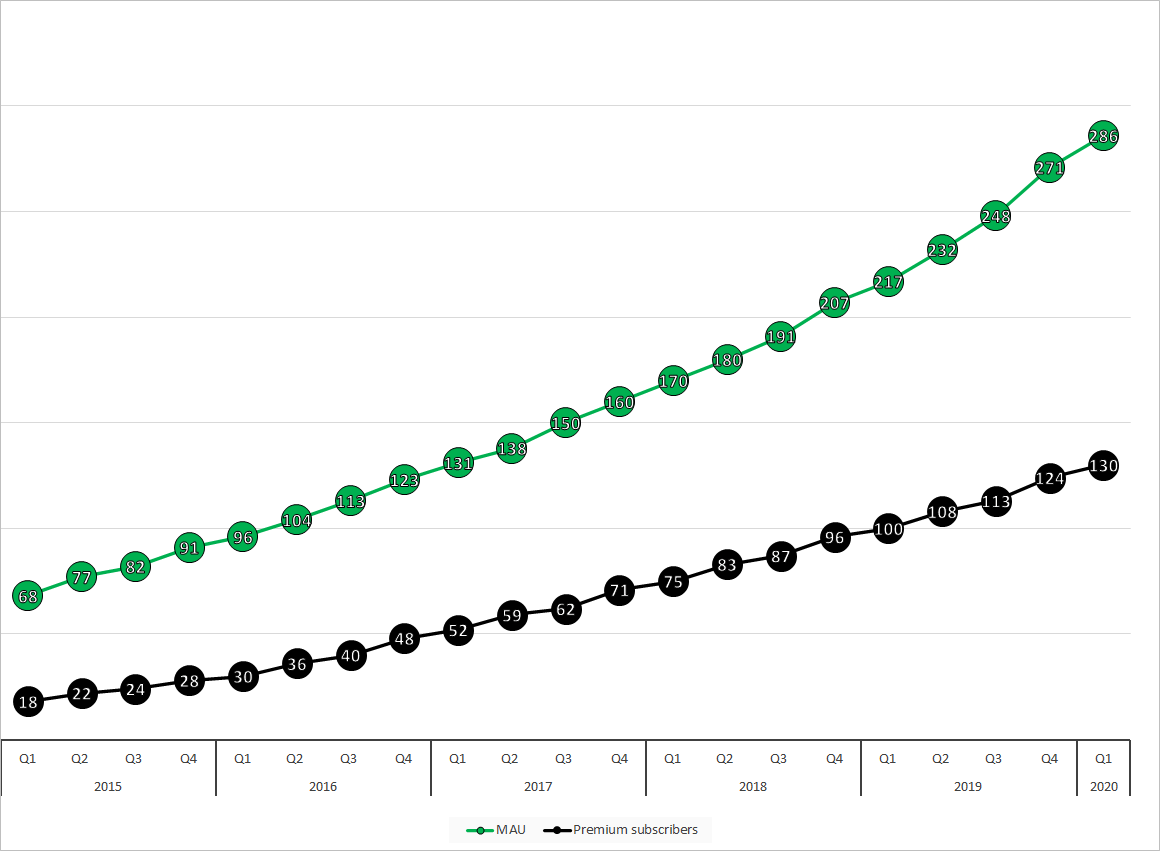
\includegraphics[scale = 0.25]{Imagens/spotify-mau-vs-subs.png}
    \caption{Número em milhões de utilizadores (verde - apenas utilizadores; preto - subscritores)} 
    \label{fig5:stats}
\end{figure}
%
%
\begin{figure} 
    \centering
    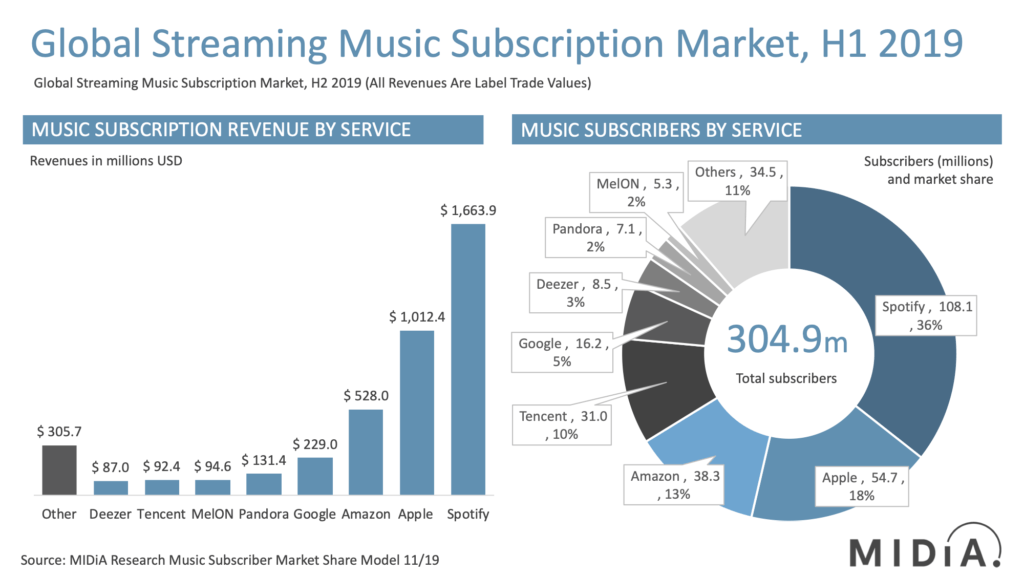
\includegraphics[width=\textwidth]{Imagens/spotify-global-market-share-1.png}
    \caption{Mercado global de plataformas musicais} \label{fig6:mercado}
\end{figure}

O \textit{Spotify} cresceu imenso na última década e não mostra sinais de abrandamento, uma vez que apresenta um crescimento de 20\% a cada ano que passa~\cite{nicklivermore&jonboon&danfallon2000}. Este crescimento passa pela quantidade de publicidade passada dentro da aplicação, um exemplo disso são os anúncios de ecrã conhecidos por \textit{Homepage Takeover} como mostra a Fig.~\ref{fig:ad} (estes anúncios são exclusivos àqueles utilizadores que não optam pela subscrição \textit{premium}). Quando se acredita no impossível, esta empresa surpreende com um tipo de publicidade diferente de qualquer outra. Esta consiste numa playlist publicitária com sons exclusivos de um determinado produto, como exemplo temos a Fig.~\ref{fig:playlist}. Deste modo, é relevante realçar o \textit{Spotify} na sua estratégia de Marketing Digital, devido ao facto de 52\% das reproduções partirem do aplicativo instalado no telemóvel e, inclusivamente, as pessoas passam em média 2 horas por dia agarradas ao telemóvel, pelo que a possibilidade de a sua estratégia chegar a um público maior é muito superior.
%
\begin{figure}
    \centering
    \begin{minipage}[b]{0.4\textwidth}
   
\includegraphics[scale = 0.5]{Imagens/admccafe.jpg}
    \caption{Exemplo de um anúncio} \label{fig:ad}
    \end{minipage}
    \hfill
    \centering
    \begin{minipage}[b]{0.4\textwidth}
    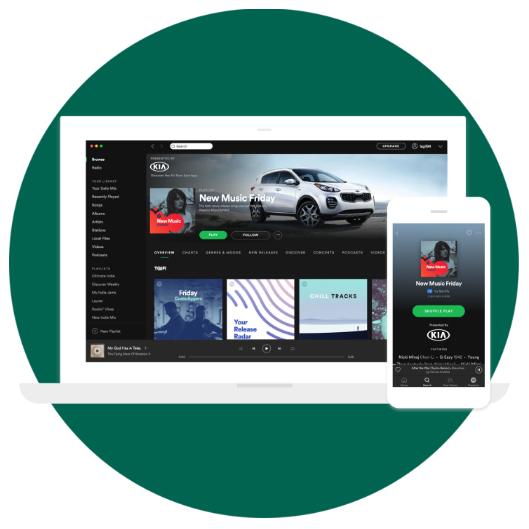
\includegraphics[scale = 0.2]{Imagens/playlistad.PNG}
    \caption{Exemplo de uma \textit{playlist} publicitária} \label{fig:playlist}
    \end{minipage}
\end{figure}
%

Agora falando das estratégias de marketing desta empresa, a maior parte da publicidade da aplicação é apresentada e divulgada em outras aplicações, em diversos sites, assim como é usual encontrar, por exemplo, nos Estados Unidos da América, mais concretamente em \textit{Nova York} - na \textit{Times Square}. Esta é também conhecida por usar os painéis da \textit{Times Square} como forma de publicidade, muitas vezes satirizando acontecimentos, tendo por base as estatísticas obtidas, de alguns ouvintes, como mostra a Fig.~\ref{fig:sátira}.

%
\begin{figure}
    \centering
    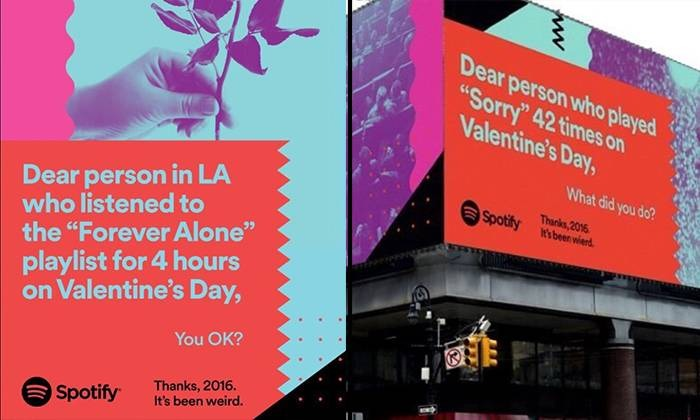
\includegraphics[width=\textwidth]{Imagens/satira.jpeg}
    \caption{Sátira} \label{fig:sátira}
\end{figure}
%



\section{Curiosidades}
A aplicação em debate apresenta diversas curiosidades, entre as quais se destaca esta altura de todos os anos, o mês de dezembro, como último mês do ano. Por volta desta época, é comum o \textit{Spotify} gerar um \textit{flashback} do ano em questão, denominado \textit{Spotify Wrapped - Listening is everything}, que consiste em informar ao utilizador o tempo em minutos que nesse determinado ano passou a ouvir música (e em que situações), o números de artistas e géneros musicais descobertos, assim como o top 5 de artistas favoritos e de músicas mais ouvidas. Apresenta estatísticas pessoais extraordinárias, como por exemplo o top de percentagem a nível mundial do top 1 de artistas mais ouvidos (de cada um) e ainda gera uma \textit{playlist} com um total de 100 músicas mais ouvidas, como mostra a Fig.~\ref{fig 8: 2020 Wrapped}

A plataforma disponibiliza um site super interessante de explorar \url{https://www.statsforspotify.com}, para que todo e qualquer ouvinte do \textit{Spotify} possa acompanhar o seu percurso individual de top de artistas e músicas dos últimos 4 meses, 6 meses ou de sempre, como mostra a Fig.~\ref{fig7:stats}

%
\begin{figure}
    \centering
    \begin{minipage}[b]{0.7\textwidth}
    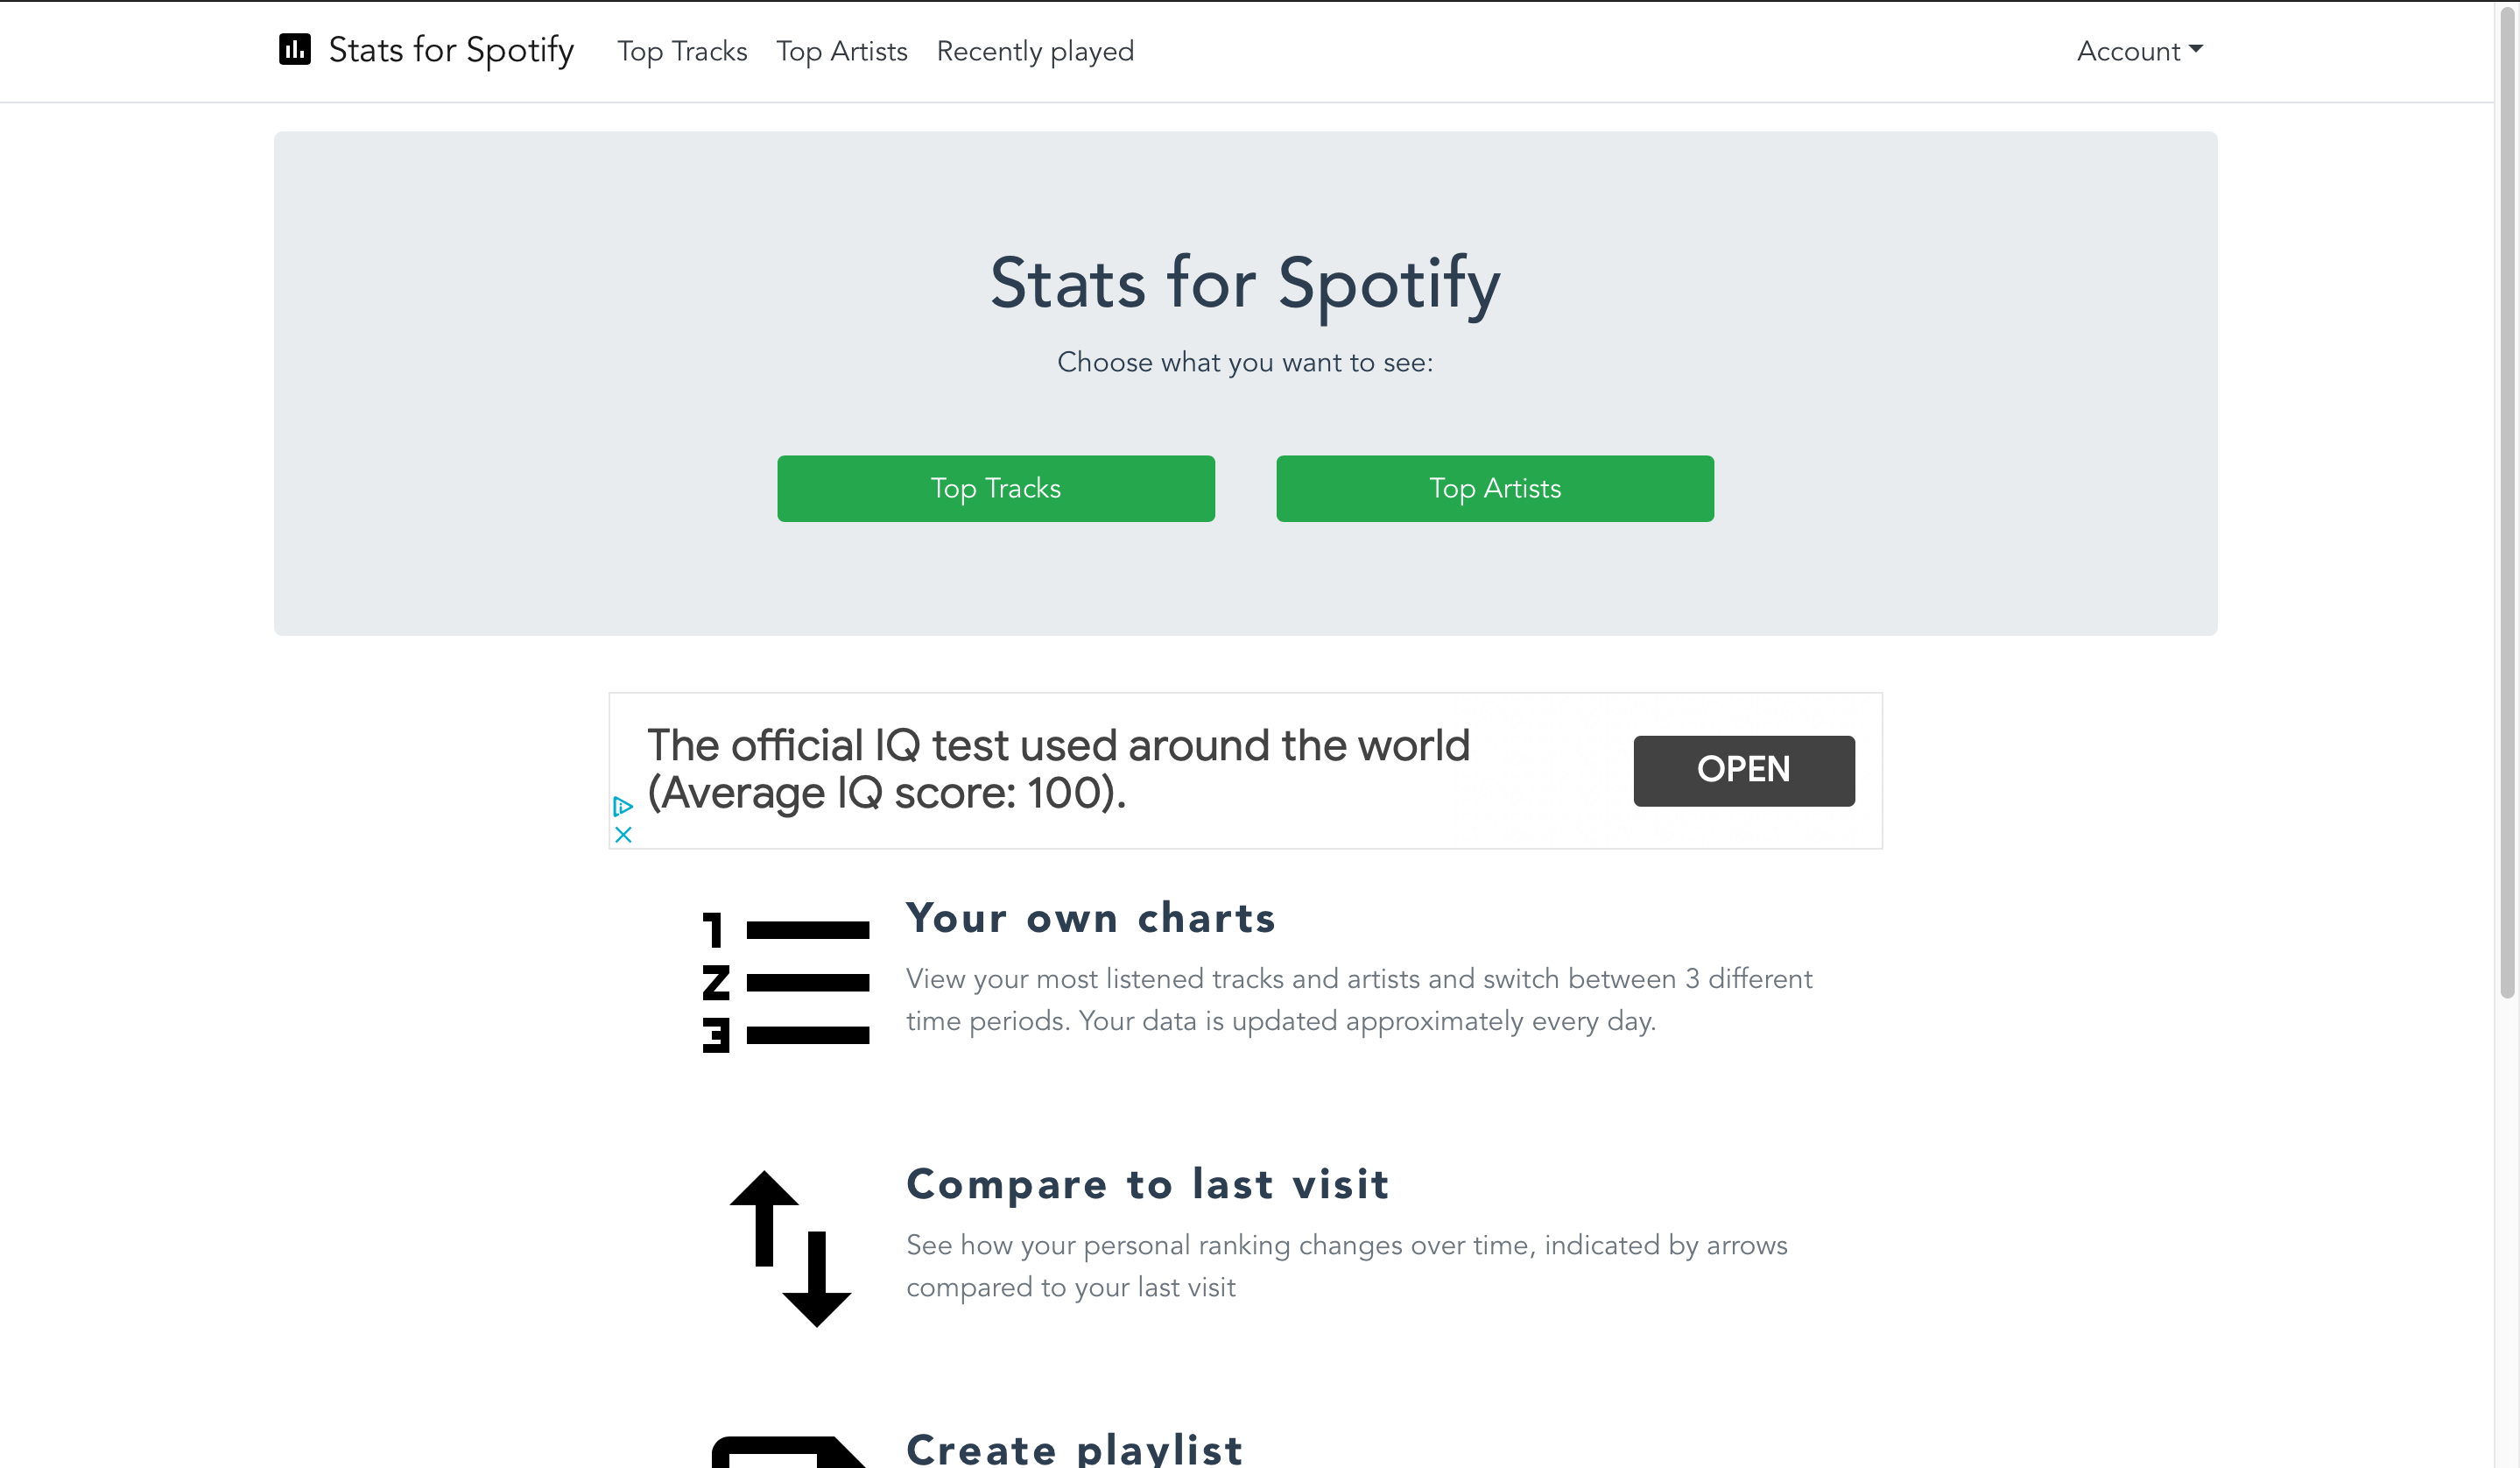
\includegraphics[width=\textwidth]{Imagens/statsforspotify.png}
    \end{minipage}
    \hfill
    \begin{minipage}[b]{0.7\textwidth}
    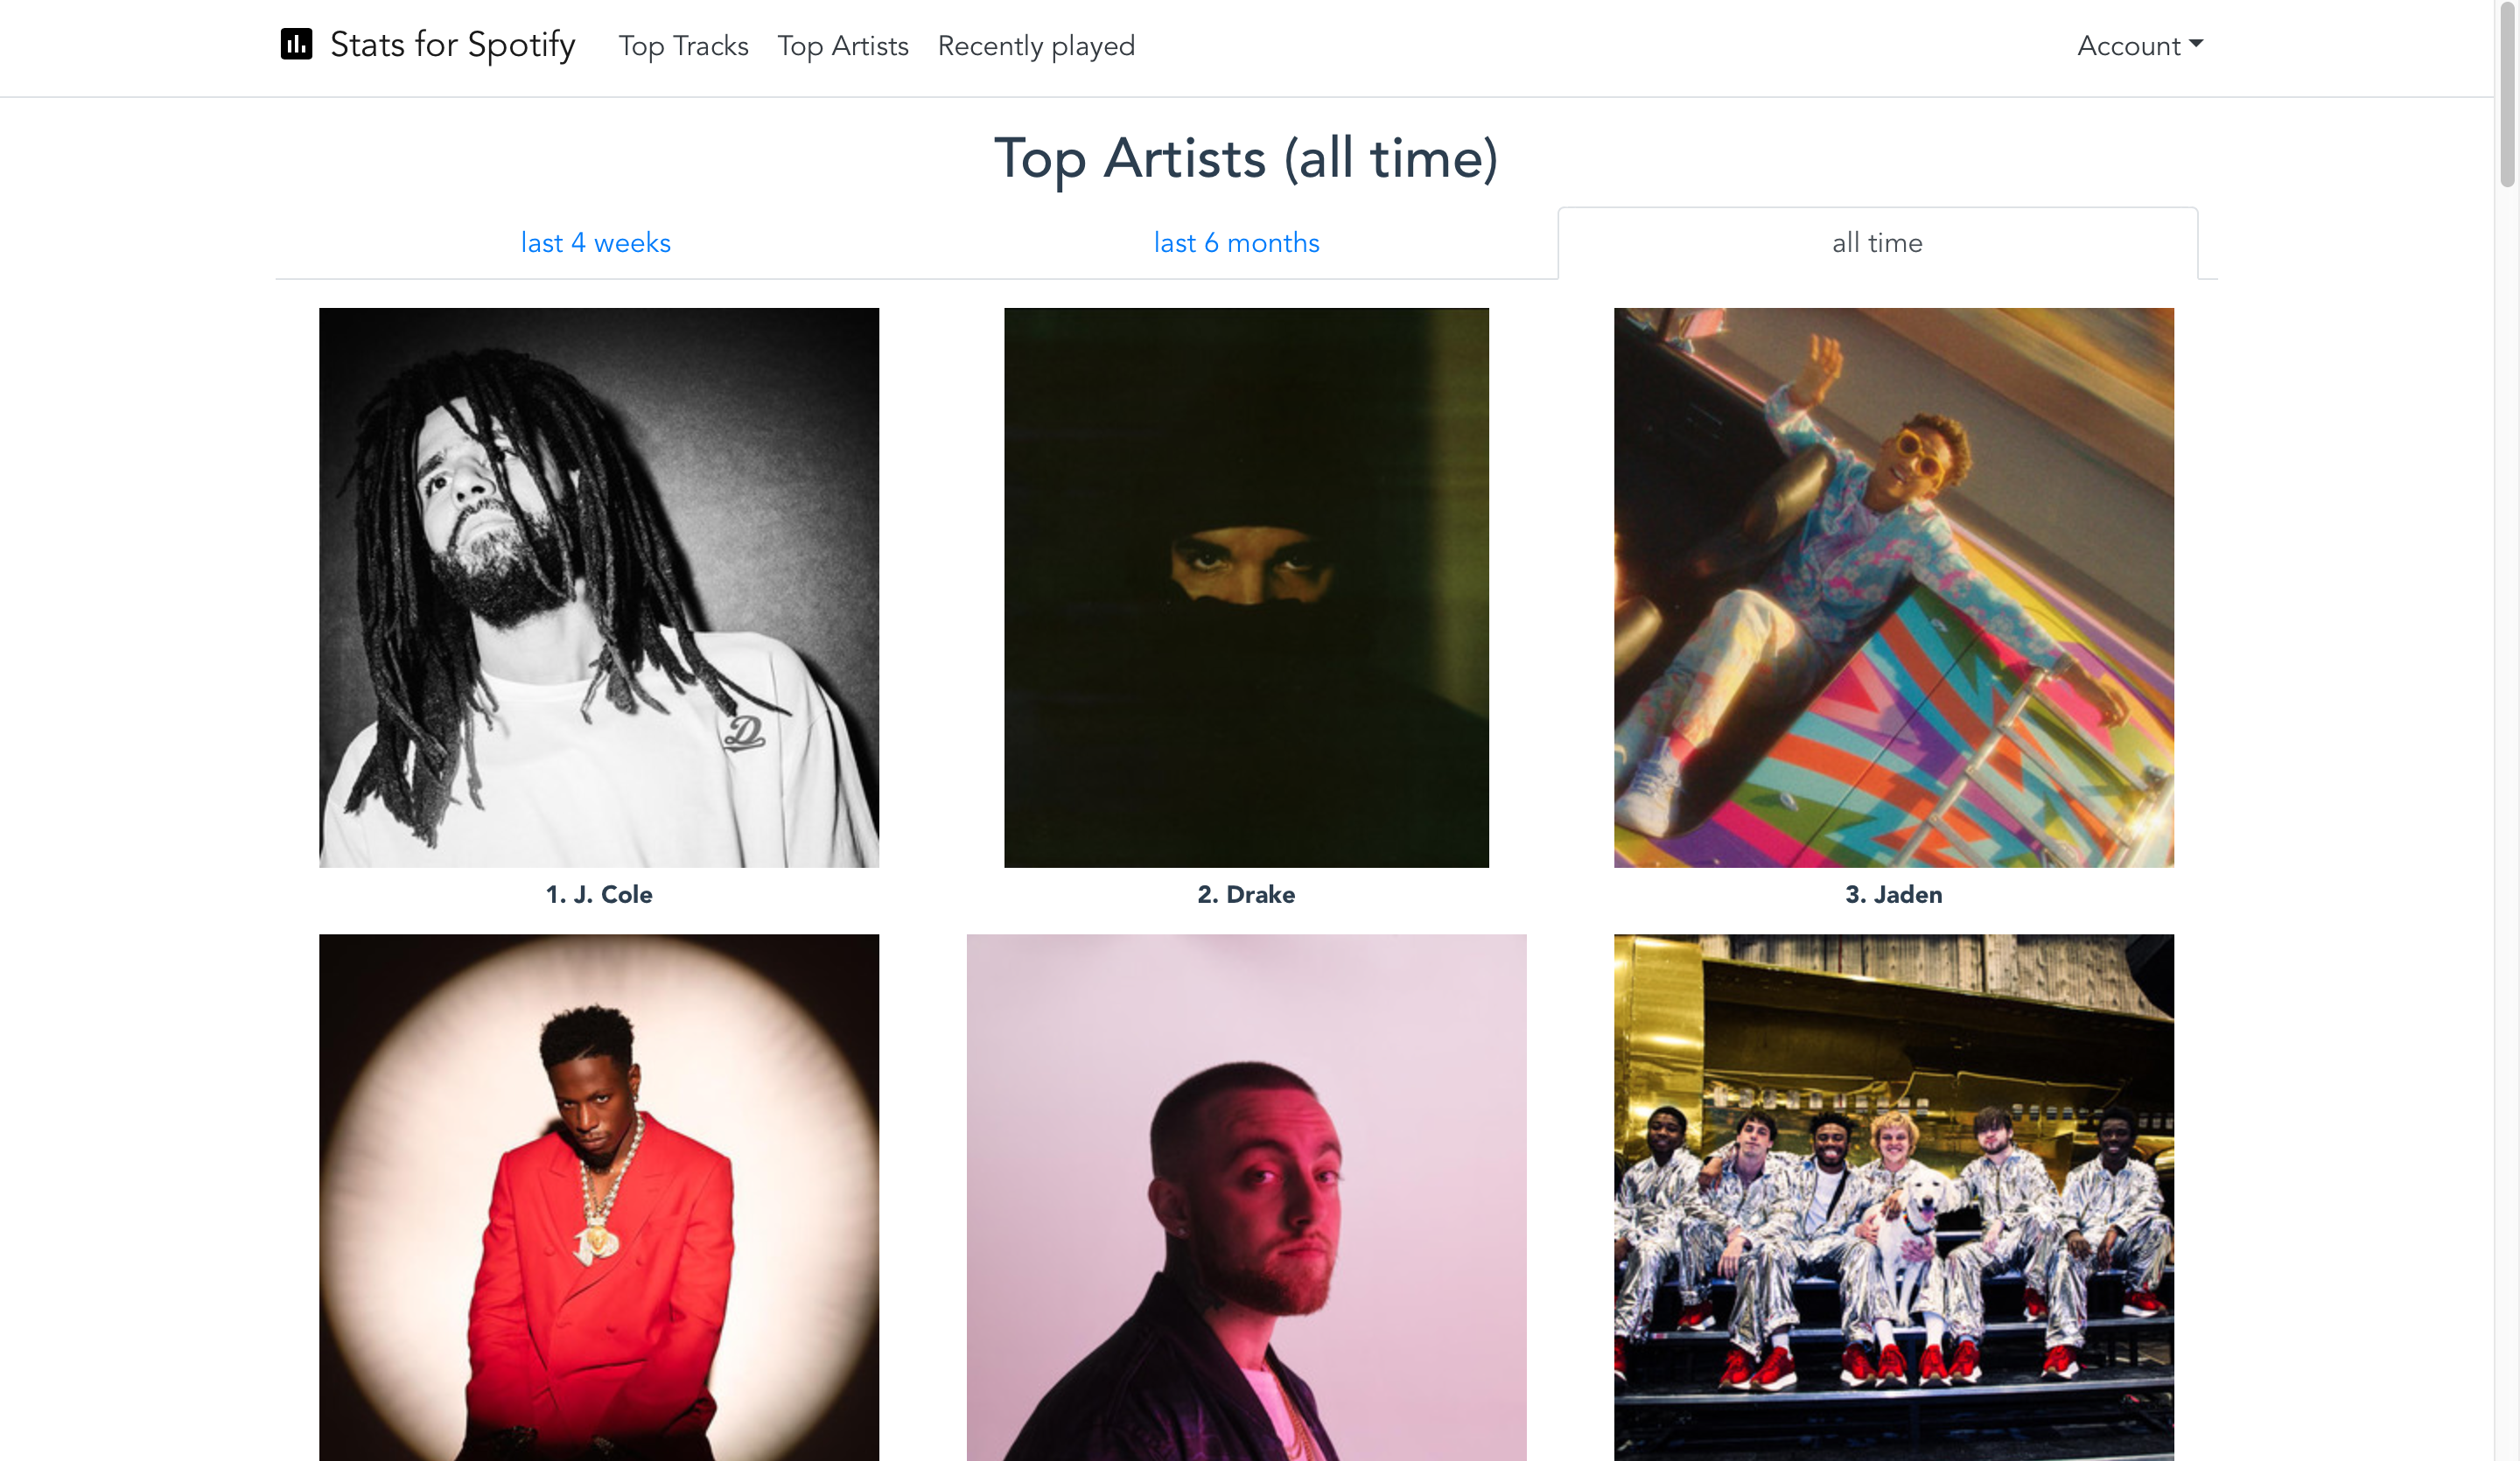
\includegraphics[width=\textwidth]{Imagens/topartists.png}
    \end{minipage}
     \hfill
    \begin{minipage}[b]{0.7\textwidth}
    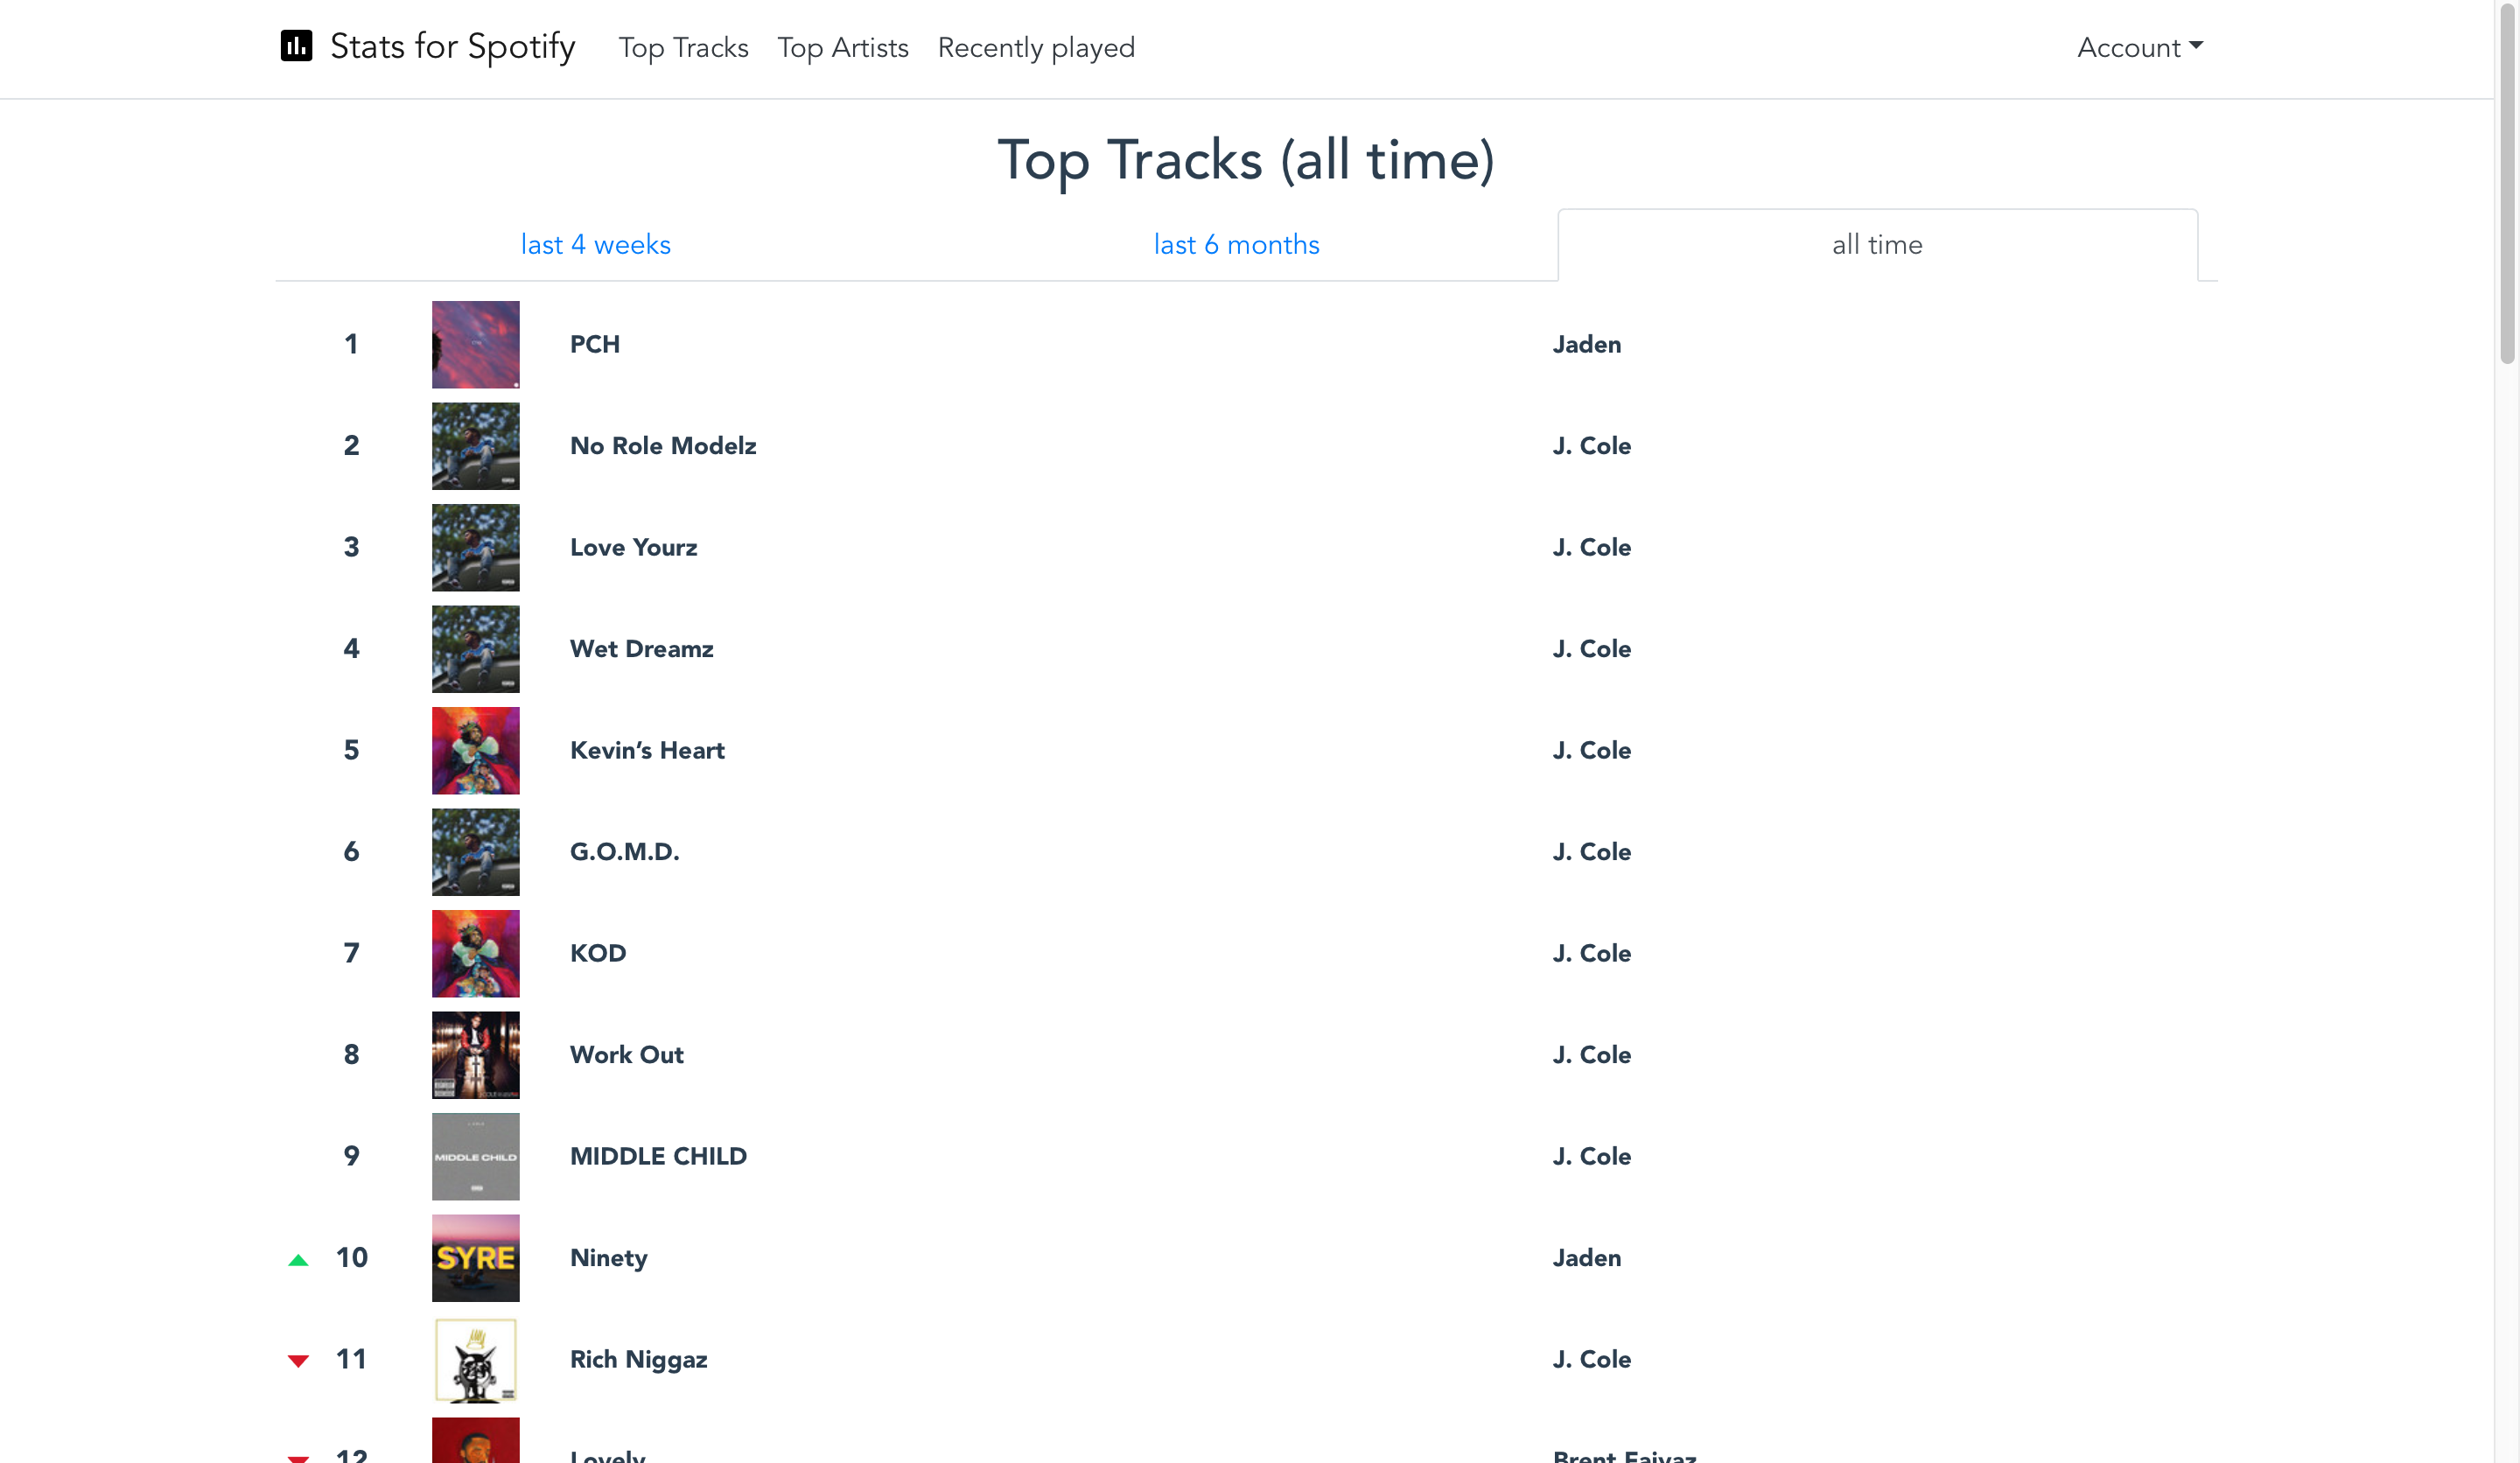
\includegraphics[width=\textwidth]{Imagens/toptracks.png}
    \end{minipage}
    \caption{\textit{Stats for Spotify}} \label{fig7:stats}
\end{figure}
%
\begin{figure}
  \centering
  \begin{minipage}[b]{0.25\textwidth}
    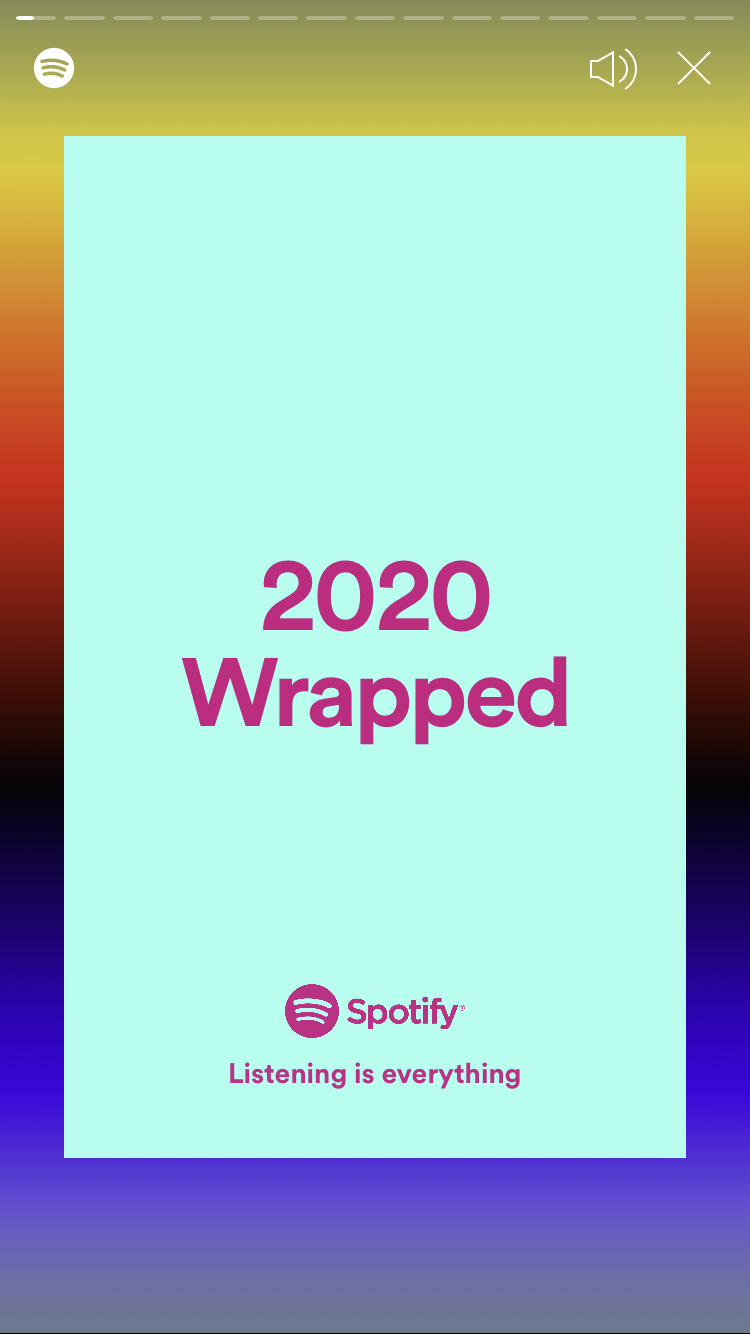
\includegraphics[width=\textwidth]{Imagens/2020.PNG}
  \end{minipage}
  \hfill
  \begin{minipage}[b]{0.25\textwidth}
    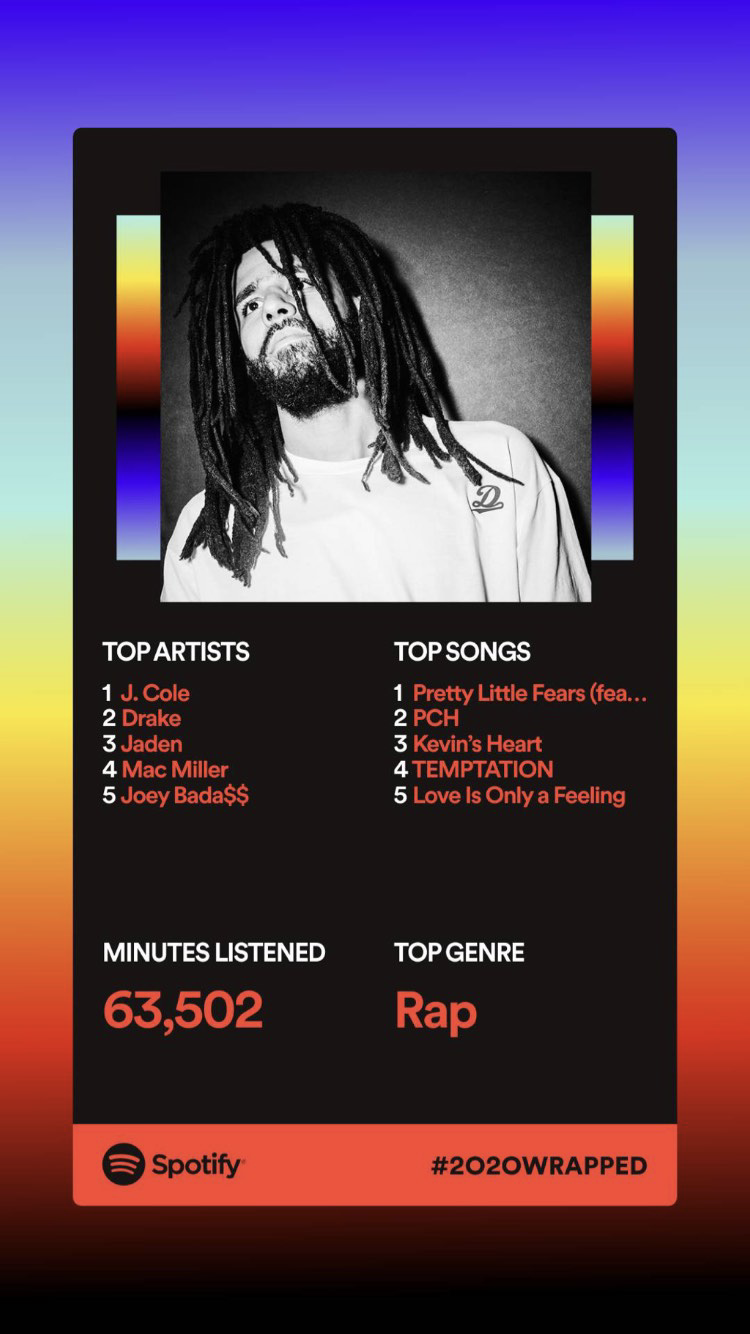
\includegraphics[width=\textwidth]{Imagens/IMG_3810.PNG}
  \end{minipage}
  \hfill
  \begin{minipage}[b]{0.25\textwidth}
    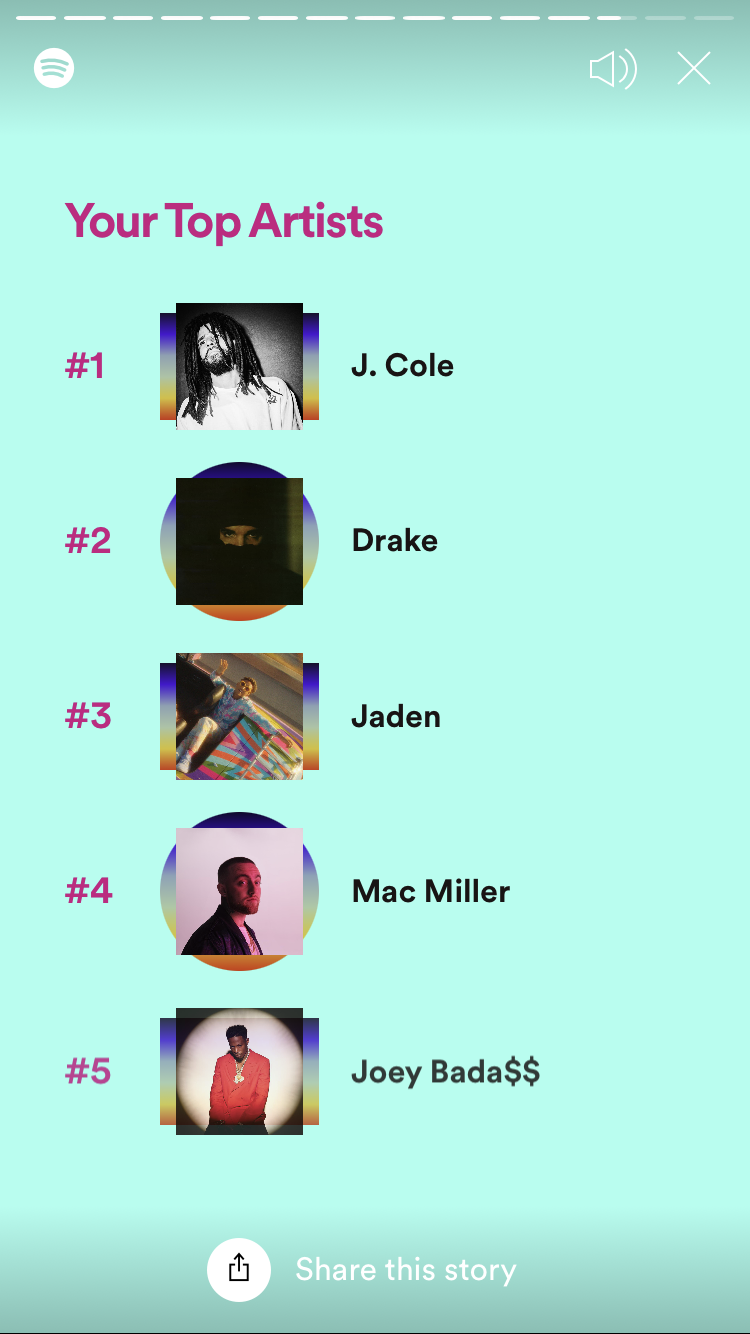
\includegraphics[width=\textwidth]{Imagens/IMG_3833.PNG}
  \end{minipage}
  \hfill
  \begin{minipage}[b]{0.25\textwidth}
    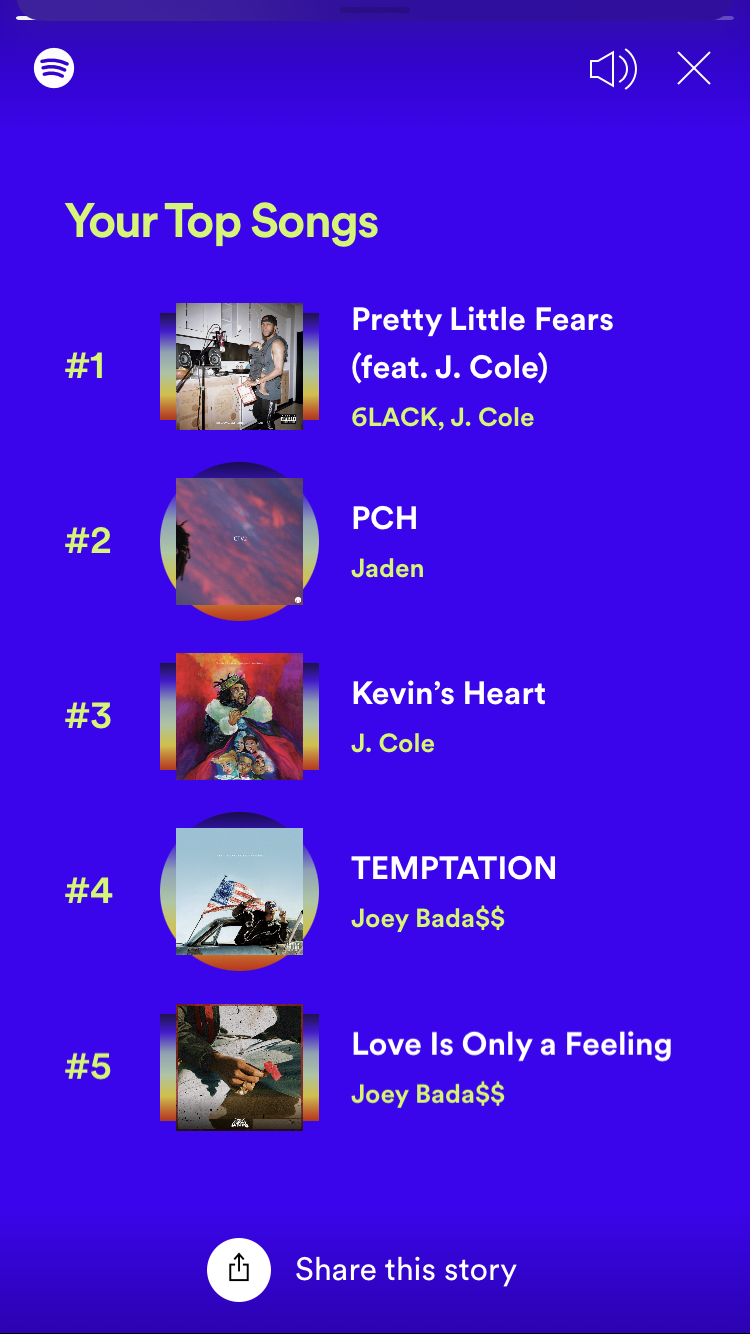
\includegraphics[width=\textwidth]{Imagens/IMG_3827.PNG}
  \end{minipage}
  \hfill
   \begin{minipage}[b]{0.25\textwidth}
    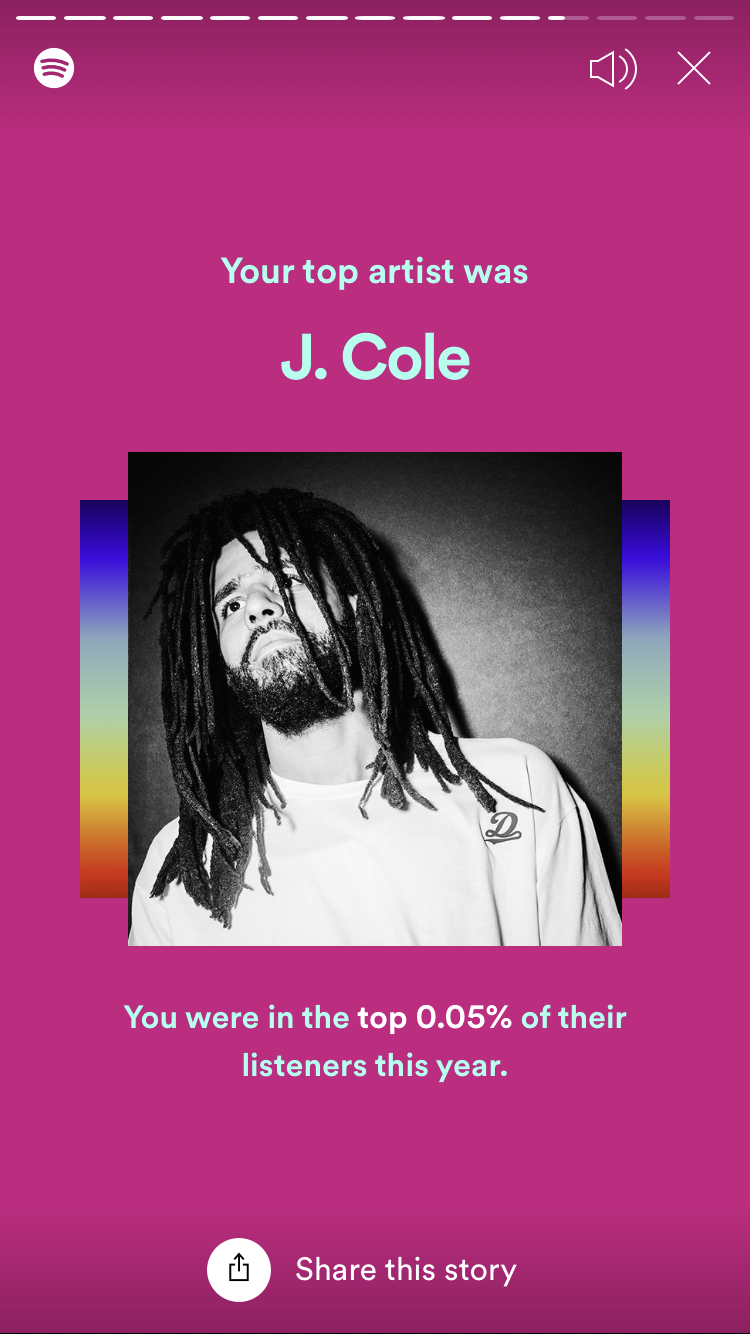
\includegraphics[width=\textwidth]{Imagens/IMG_3831.PNG}
  \end{minipage}
  \hfill
  \begin{minipage}[b]{0.25\textwidth}
    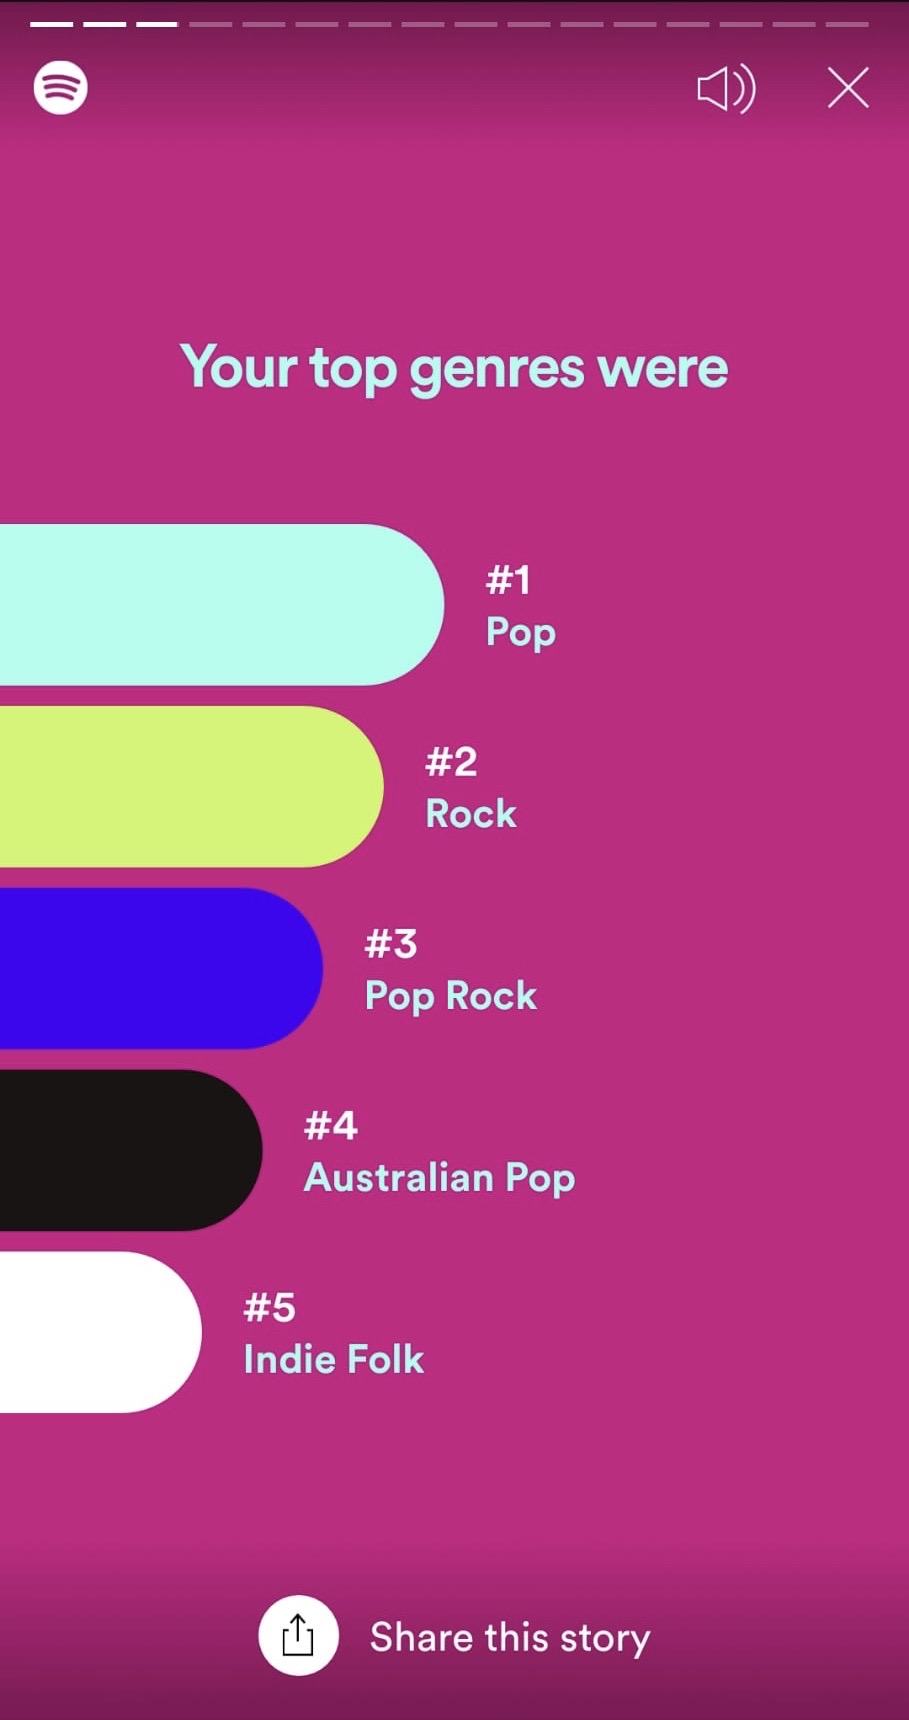
\includegraphics[width=\textwidth]{Imagens/generos.jpeg}
  \end{minipage}
   \hfill
  \caption{2020 Wrapped }
  \label{fig 8: 2020 Wrapped}
\end{figure}



\chapter{Conclusões}
\label{chap.conclusao}
Deste modo, já é possível responder às \textbf{problemáticas} apresentadas inicialmente: 
\begin{quote}
``\emph{Será que o Spotify é a plataforma digital de áudio de alta qualidade mais usada e mais apetecida pelo público? E porquê?}'' - IS \& JF
\end{quote}

Como se pode constatar o que foi abordado neste relatório, é claramente visível a predominância do Spotify nas vidas de quem o escolhe utilizar, assim como a predominância em relação às concorrentes indústrias de \textit{streaming} a nível mundial, não só em números como em qualidade e apresentação. É, de facto, incrível como uma simples e única aplicação revolucionou o mundo da música, principalmente devido ao impacto e à facilidade de prestação de se adequar às preferências e gostos dos seus utilizadores. Ficou bastante clara a importância da música para cada indivíduo diariamente, em qualquer altura do dia, e o facto de ter efetivamente acesso a ela 24/7 (24h por dia, 7 dias por semana). Atendendo a este facto, a aplicação impôs-se acima da concorrência apresentando o modelo da \textit{app} para qualquer tipo de dispositivo, quer este seja computador, telemóvel, tablet, televisão \dots ~\cite{andrewtseng2020}. É de extrema relevância abordar o facto como o Spotify aproveitou estes tempos de pandemia e do período de confinamento global da população para obter lucros e números nunca antes vistos, uma vez que estando confinado e não tendo nada para fazer ou até, no caso de certas pessoas, durante atividades mais aborrecidas como tarefas domésticas e estudar, fornece uma forma de motivação, para acalmar e, de certa forma, desconectar-se ou até mesmo ``esquecer'' por momentos a gravíssima situação atual em que nos encontramos.

Por fim, e como forma de colmatar este trabalho, estima-se que num futuro próximo o Spoptify tenha um crescimento ainda mais significativo ($2x$, $3x$, \dots quem sabe?) que possui atualmente esta empresa (quando se fala num futuro próximo, refere-se a 5/10 anos). A tecnologia está a evoluir de forma exponencial a cada ano que passa, e a Humanidade, quer queiramos quer não, vai sentir o impacto desta evolução, das mudanças e propostas inovadoras que vão de certeza surgir nos próximos anos. A vida é mesmo assim: feita de mudanças. E é preciso sermos suficientemente inteligentes para encarar os novos desafios com que a Realidade nos presenteia todos os dias. Citando Albert Einstein:

\begin{quote}
``\emph{The measure of intelligence is the ability to change}.''    
\end{quote}


\chapter*{Contribuições dos autores}
O trabalho foi desenvolvido pelos dois membros de igual esforço e dedicação pelo que tanto JF e IS contribuíram de igual forma para este relatório.
Cada um foi responsável, numa fase inicial, pela escrita repartida de 2 capítulos, com um acréscimo do resumo e da conclusão no final (sendo feita esta divisão em 3 tarefas para cada membro). Em fases posteriores, houve um crescente trabalho colaborativo na elaboração e edição do documento {\LaTeX}.

 Deste modo, a percentagem de contribuição atribuída será estimada de $50\%$ para ambas as partes.


%%%%%%%%%%%%%%%%%%%%%%%%%%%%%%%%%
\chapter*{Acrónimos}
\begin{acronym}
\acro{ua}[UA]{Universidade de Aveiro}
\acro{miect}[MIECT]{Mestrado Integrado em Engenharia de Computadores e Telemática}
\acro{glisc}[GLISC]{Grey Literature International Steering Committee}
\acro{inc}[INC]{Incorporating companies}
\end{acronym}


%%%%%%%%%%%%%%%%%%%%%%%%%%%%%%%%%
\printbibliography

\end{document}

